\documentclass[11pt,a4paper]{article}
\usepackage[T1]{fontenc}
\usepackage[utf8]{inputenc}
\usepackage{lmodern}
\usepackage{mathpazo}
\usepackage{amsmath,amssymb,amsthm,mathtools}
\usepackage[margin=27mm,headheight=14pt]{geometry}
\usepackage{microtype,booktabs,array,longtable,enumitem}
\usepackage{placeins}
\usepackage{xcolor,graphicx,tikz,fancyhdr,fancyvrb}
\usetikzlibrary{arrows.meta,positioning,calc}
\usepackage{xurl}
\usepackage[colorlinks=true,linkcolor=navy,citecolor=navy,urlcolor=navy]{hyperref}
\usepackage[nameinlink,noabbrev]{cleveref}
\definecolor{navy}{HTML}{173D59}
\definecolor{teal}{HTML}{167C80}
\definecolor{muted}{HTML}{53616C}
\hypersetup{pdftitle={Deferred Forests and Exceptional Incidence for Compressed Unknot Hierarchies},pdfauthor={ProveIt research continuation, prepared with ChatGPT Pro},pdfsubject={Exact primal-forest elimination, parameterized dual-forest selection, and authenticated native experiments}}
\newtheorem{theorem}{Theorem}[section]
\newtheorem{lemma}[theorem]{Lemma}
\newtheorem{proposition}[theorem]{Proposition}
\newtheorem{corollary}[theorem]{Corollary}
\theoremstyle{definition}
\newtheorem{definition}[theorem]{Definition}
\newtheorem{assumption}[theorem]{Assumption}
\theoremstyle{remark}
\newtheorem{remark}[theorem]{Remark}
\newcommand{\NN}{\mathbb N}
\newcommand{\calR}{\mathcal R}
\newcommand{\code}[1]{\texttt{#1}}
\DeclareMathOperator{\Reach}{Reach}
\DeclareMathOperator{\Bell}{Bell}
\DeclareMathOperator{\supp}{supp}
\DeclareMathOperator{\cl}{cl}
\setlist{topsep=4pt,itemsep=3pt,parsep=0pt}
\setlength{\parskip}{3pt}
\setlength{\emergencystretch}{2em}
\pagestyle{fancy}
\fancyhf{}
\fancyhead[L]{\small\color{muted}ProveIt research continuation}
\fancyhead[R]{\small\color{muted}Deferred forests}
\fancyfoot[C]{\thepage}
\renewcommand{\headrulewidth}{0.3pt}
\DefineVerbatimEnvironment{Code}{Verbatim}{fontsize=\small,frame=single,rulecolor=\color{muted},framesep=7pt}
\title{\color{navy}\bfseries Deferred Forests and Exceptional Incidence\\[5pt]
\Large Exact local reductions for compressed unknot hierarchies}
\author{Research continuation for Vladimir Reshetnikov's ProveIt project\\[3pt]
\small Prepared with ChatGPT Pro; independent mathematical review invited}
\date{12 October 2026\\[4pt]\small Repository baseline: \texttt{c6d0ec8aa0b6308310ab6c081ba29d8bc363ede5}}

\begin{document}
\maketitle
\begin{abstract}
We eliminate one exponential search variable in the repository's raw
geometric handle-cancellation problem.  If two-handle rows are literal
closed walks in the zero/one-handle graph, column-leaf peeling on the full
incidence matrix preserves the original graph components when its graph
pivots are deleted.
A spanning forest can therefore be chosen \emph{after discovery}, avoiding
every pivot, and contracted \emph{before replay}.  This is an exact test
over all primal forests for complete raw positive-singleton cancellation;
a stopping set provides a universal refusal witness for this restricted
model.  The result also applies to the authenticated finite bundle-boundary
matrix when all annular rows are assembled first.

For the remaining dual-forest choice, we prove an exact finite selector
with running time $2^{O(u\log(u+2))}\operatorname{poly}(N)$, where $u$ counts
rows incident with active columns supported on more than two rows.  The
proof compresses ordinary implications onto this exceptional interface and
enumerates partial set partitions, using at most $\Bell(u+1)$ polynomial
graphic/partition matroid-intersection calls.  For the original native
core columns, the established three-occurrence bound implies $u\le3k$.

An additive implementation increases historical whole-cut certificate
coverage from $92/106$ to $99/106$, and additional-case coverage from
$10/14$ to $12/14$, with all 213 old/new positive outputs independently
replayed.  The standalone dual selector agrees with exhaustive oracles on
50,658 finite instances.  We supply full proofs, a geometric all-size
separation family, raw experiments, source-bound certificates, a patch,
and a prioritized research programme.  These are local mathematical and
implementation advances.  We do not claim a complete quasi-polynomial
unknot recognizer or a global logarithmic exceptional-interface bound.
\end{abstract}
\clearpage
\tableofcontents
\clearpage
\section{Scope, provenance, and the precise contribution}
\label{sec:scope}

The engineering objective is to make compressed normal cuts useful inside
an eventual fast hierarchy algorithm for unknot recognition.  A terminal
operation already present in ProveIt takes a triangulation and a normal
surface in binary coordinates, builds source-authenticated compressed
geometry, and tries to certify the genera and multiplicities of all
handlebody components of the cut.  Its output is deliberately partial:
a successful certificate is independently replayable; a failed search is
\code{INCONCLUSIVE}.  The operation is not itself a decision procedure for
all knots, nor does a handlebody census alone encode every marked boundary
map needed to continue a hierarchy.

We work at commit
\begin{center}\small
\texttt{c6d0ec8aa0b6308310ab6c081ba29d8bc363ede5}.
\end{center}
The inspected material includes the maintained \code{fast} implementation,
the synthesis notes, and all five archives in \code{docs/incoming} at this
commit.  The delivered patch is against that revision, not a moving branch.
The source audit records the hashes of the incoming archives and changed
modules.  No repository publication or merge is part of this package.

\subsection{What the preceding research already established}

The incoming material is substantial.  In particular, the following are
inputs to this continuation, not new claims made here.

\begin{enumerate}
\item \emph{Positive cancellation.}  Complete elimination of the rows of
a nonnegative occurrence matrix by positive singleton pivots is equivalent
to column-leaf peeling.  A greatest stopping set is the obstruction, and
immutable source entries admit a sparse queue and timestamp replay
\cite{IncomingPositive}.  We reprove the required statement in
Section~\ref{sec:raw} so the new argument is self-contained.
\item \emph{Dual normalization.}  The native top handles can be removed
using a source-authenticated dual spanning tree, relative to the exposed
ports.  For active columns on at most two rows, the remaining tree-selection
problem has a polynomial graphic/partition matroid formulation.  Original
native source columns have at most three literal occurrences; their odd
supports obey the dual cycle condition \cite{IncomingDualNormalization}.
\item \emph{Other compressed infrastructure.}  Component gauges, cut
atlases, occurrence-preserving flag regularization, weighted forest
heuristics, and homological progress certificates were developed in the
other incoming notes \cite{IncomingGauges,IncomingFlags,IncomingProgress}.
They remain relevant to successor construction and to other move classes.
\end{enumerate}

The maintained code at our baseline already incorporates several of these
ideas, including a deterministic breadth-first dual-tree reduction.  Its
historical whole-cut census coverage is $92/106$.  Reimplementing that
reduction or rediscovering the matrix-only peeling theorem would not be a
new contribution.

\subsection{New results relative to the inspected baseline}

Our first result uses geometry that the matrix-only model discarded:
attaching curves are closed walks in the primal graph.  It proves that
all useful peeling pivots can be kept outside some spanning forest.  Thus
the primal forest can be eliminated as a search variable, even though its
canonical choice can destroy all apparent progress.  The constructive
proof gives a strictly larger native certificate class without introducing
word reduction, speculative handle slides, or a new topology oracle.

Our second result addresses the remaining high-support columns in dual
selection.  Their incident rows form a finite interface.  Ordinary
implications can be compressed onto that interface, and a successful tree
needs at most one additional witness for each interface row.  Enumerating
\emph{how targets share witnesses}, rather than enumerating all choices of
tree edges, gives a Bell-number parameter dependence.  The classical
matroid machinery is reused; the exceptional-interface reduction is the
new part.

A third contribution is the exact geometric separation family of
Section~\ref{sec:forest-separation-family}.  It identifies a genuine failure
of a fixed forest policy and an exponential candidate space, while making
no lower-bound claim against every possible algorithm.  The implementation
and the native experiments then test whether the first theorem helps the
actual source geometry.  It does: nine additional whole-cut packets are
certified across the two supplied corpora.

Here and throughout, ``new'' means absent from the inspected repository
and incoming research and developed in this continuation.  We have not
established a comprehensive priority claim across all of low-dimensional
topology, hypergraph peeling, matroid activation, and sparse elimination.
The mathematical statements are proved in the article and subjected to
separate proof review and implementation audits; they have not been
formalized in a proof assistant or externally peer reviewed.

\subsection{Relation to Lackenby's announced target}

The 2021 talk materials announce $n^{O(\log n)}$ unknot recognition; an
Oxford compressed handout separately displays a weaker
$n^{O(\log^2 n)}$ estimate.  Both are quasi-polynomial, but their exponents
should not be conflated \cite{Lackenby2021,LackenbyOxford2021}.
Lackenby's July 2026 paper gives the hierarchy algorithm and explicitly
leaves speed-up to future work \cite{Lackenby2026}.  Its Theorem~6.2 already
constructs a nonseparating oriented normal surface in polynomial time
under its handle hypotheses.  Proposition~9.1 bounds the relevant loop
count by $L(g+1)^L$; the refined construction has length at most $4c_q$.
Theorem~11.3 controls uniform handle type.  Proposition~14.2 and
Theorem~14.4 give compressed successor and parallelity-bundle constructions
under their stated geometric hypotheses.  These are established local
results, not open problems solved by this package.

Our target is to turn applicable theory into a source-authenticated,
bounded-cost implementation and to improve the local terminal and
normalization operators.  Neither a faster terminal census nor a
parameterized forest selector supplies the missing global hierarchy bound.
Section~\ref{sec:complexity} writes those remaining obligations explicitly.

\subsection{Parameters and trust boundaries}

We distinguish the crossing count $n$ of a knot diagram from the encoded
size $N$ of a particular finite graph/matrix or compressed cut state.
A normal weight $W$ is different again: its bit length is logarithmic in
$W$.  A polynomial in expanded normal weight is generally unusable for
the desired asymptotic goal.

The finite theorems accept exact integer matrices and graphs.  A topology
application must additionally authenticate that these objects arise from
the specified handles, attaching charts, and legal port-preserving moves.
A matrix with the right parity is not automatically a native normal cut.
This distinction applies especially to the triangle witness in
Section~\ref{sec:exceptional}: it tests a constrained finite class, while
the nine new native certificates have full source records and independent
whole-cut replay.

\section{The raw cancellation invariant}
\label{sec:raw}

This section records the exact algebraic prerequisite from the preceding
positive-cancellation work \cite{IncomingPositive}.  The use of unsigned
literal occurrences is essential.  These counts record intersections with
specified belt discs; they are not exponent sums of freely reduced words.

\begin{definition}[Positive singleton pivot and stopping set]
Let $A=(a_{rc})$ be a finite nonnegative integer matrix with rows $R$ and
columns $C$.  A positive singleton pivot chooses $(r,c)$ with $a_{rc}=1$,
deletes row $r$ and column $c$, and changes each surviving entry to
\[
 a'_{id}=a_{id}+a_{ic}a_{rd}\qquad(i\ne r,\ d\ne c).
\]
A nonempty set $S\subseteq R$ is a \emph{stopping set} if
\[
 s_c:=\sum_{r\in S}a_{rc}\in\{0\}\cup\{2,3,\ldots\}
 \quad\text{for every }c\in C.
\]
A \emph{column leaf} has total live column occurrence one.  Pivoting on
it creates no fill in the surviving rows and is called a peeling move.
\end{definition}

The formula deliberately has a plus sign.  It is the conservative raw
intersection update: algebraic cancellation of opposite letters is not
part of this model.  The theorem below cannot be extended to arbitrary
subtractive elimination merely by reusing its proof.

\begin{lemma}[A stopping set survives positive pivots]
\label{lem:stopping-invariant}
If $A$ contains a stopping set, then every legal positive singleton pivot
leaves a nonempty stopping set on surviving rows.
\end{lemma}
\begin{proof}
Let $(r,c)$ be the pivot and let $S$ be a stopping set.  If $r\notin S$,
retain $S$.  For each surviving column $d$ its new total is
$s_d+s_c a_{rd}$.  If this is positive, either $s_d\ge2$ or
$s_c a_{rd}\ge2$, so it is not one.

If $r\in S$, the pivot entry is one and $s_c\ne1$, hence $s_c\ge2$.
Another row of $S$ meets $c$, so $S'=S\setminus\{r\}$ is nonempty.  Its
new total in column $d\ne c$ is
\[
 \sum_{i\in S'}a'_{id}
 =s_d-a_{rd}+(s_c-1)a_{rd}
 =s_d+(s_c-2)a_{rd}.
\]
If $s_d=0$, then $a_{rd}=0$ and the total is zero.  Otherwise $s_d\ge2$
and the total is at least two.  Thus $S'$ is a stopping set.
\end{proof}

\begin{theorem}[Complete raw cancellation equals peeling; prior result]
\label{thm:raw-completeness}
For every finite nonnegative integer matrix, the following are equivalent:
there exists a complete positive singleton sequence; column-leaf peeling
deletes every row; and there is no nonempty stopping set.  Peeling's
terminal row set is independent of queue order and is the greatest
stopping set, with the empty set allowed as the greatest residual.
\end{theorem}
\begin{proof}
A nonempty stopping set excludes a complete positive sequence by
Lemma~\ref{lem:stopping-invariant}.  If peeling stops with live rows, their
column totals are zero or at least two, so these rows form a stopping set.
Consequently the absence of stopping sets forces peeling to finish, and
peeling itself is a positive singleton sequence.

Any stopping set in the original matrix survives every peeling move
unchanged: a live column of total one cannot meet it.  Hence every original
stopping set is contained in the terminal row set.  That terminal set is
itself a stopping set when nonempty.  It is therefore the greatest one and
does not depend on the order of valid leaves.  Equivalently, unions of
stopping sets are stopping sets: a column meeting the union meets one of
its stopping subsets, which already contributes at least two.
\end{proof}

\begin{corollary}[Heredity under row deletion]
\label{cor:row-heredity}
Every row restriction of a completely peelable matrix is completely
peelable.
\end{corollary}
\begin{proof}
A stopping subset in the restricted matrix would be exactly the same
stopping subset in the original matrix.  Apply
Theorem~\ref{thm:raw-completeness}.
\end{proof}

Heredity is why a successful independent set of dual deletions can later
be extended to a spanning tree.  It does not say that an arbitrary primal
column deletion preserves success; deleting columns can remove the only
available leaves.  The new geometric theorem repairs precisely that
asymmetry.

\subsection{Saturation and immutable-source replay}

The map $x\mapsto\min\{2,x\}$ preserves whether a nonnegative sum or
product is zero, one, or at least two.  Therefore all pivot-admissibility
and stopping-set decisions can use the three values $0,1,2^+$ without
expanding large counts.  In contrast, this saturation does not preserve
parity: three becomes two.  Geometric parity conditions must be proved on
the uncapped source occurrences first.

During peeling, source coefficients never change.  Keep, for each column,
the number of remaining incident rows and the exclusive-or of their
identifiers.  If there is one owner and its source coefficient is one,
the column is a leaf.  Deleting that row updates each incident column
once.  With indexed adjacency lists this is
$O(|R|+|C|+I)$ work and storage, where $I$ is the number of nonzero
incidences.  Dictionary lookup, label encoding, and graph construction
costs are separate implementation considerations.

A positive certificate lists distinct row/column pivot pairs.  A checker
can validate them directly against immutable source rows, or use the
existing timestamp criterion: at the deletion time of row $r$, every
other owner of its chosen column must already be gone, and the coefficient
at $r$ must be one.  Successful production does not authorize a checker
to trust an unauthenticated occurrence matrix.

\subsection{Why signed homology is insufficient}

A curve traversing a belt disc three times can have algebraic intersection
one.  Its raw count is still three, so it is not a geometric singleton in
the current charts.  Likewise, a determinant equal to one can certify a
homological condition without exhibiting the disjoint attaching curves
needed for handle cancellation.  The incoming homological progress work
can guide surface choices, but its output cannot be silently substituted
for the raw matrix in this theorem.  Later sections discuss a different,
carefully scoped terminal use of verified group presentations.

% Article fragment.  Requires amsmath, amssymb and theorem environments.
\section{Postponing the lower forest eliminates a search variable}
\label{sec:deferred-primal-forest}

The previous complete dual-forest search held the zero/one forest fixed.
The previous weighted-tree proposal alternated additive optimizations of
both forests.  For the specific objective of \emph{complete raw one/two
cancellation}, however, a different argument eliminates the lower-forest
search entirely.  The producer should first find column leaves in the full
source incidence matrix, and only then choose a zero/one forest that avoids
its pivots.  The actual geometric certificate still contracts this chosen
forest \emph{before} performing its one/two cancellations.  Only discovery
is postponed; no commutation of geometric moves is assumed.

\subsection{The graph constraint that the matrix-only model forgets}

Let $G=(V,E)$ be a finite multigraph, with loops and parallel edges allowed.
Write $c(G)$ for its number of connected components.  A spanning forest
always spans each original component.  Let $R$ be a finite row set, and let
$J$ be a disjoint set of auxiliary columns.  Consider a nonnegative integer
matrix
\[
 N=(n_{rx})_{r\in R,\ x\in E\sqcup J}.
\]
Assume that, for each row $r$, its restriction $(n_{re})_{e\in E}$ is the
literal edge-occurrence vector of a closed walk in $G$.  A union of closed
walks also suffices.  An empty restriction is permitted when a row has only
auxiliary columns.  Equivalently for the argument below, it suffices that
the uncapped occurrence vector reduce modulo two to a graph cycle:
\[
 \sum_{e\ni v} n_{re}=0\pmod 2 \qquad(v\in V),
\]
where a loop contributes twice.  One must formulate this condition before
saturation: replacing a coefficient three by two preserves singleton tests
but not parity.

A \emph{column-leaf move} chooses a live column $x$ for which
\[
 \sum_{r\in R_{\mathrm{live}}}n_{rx}=1.
\]
It deletes its unique incident row and deletes column $x$.  Other entries
are unchanged.  All earlier pivot columns have zero occurrence in every
later live row.  Thus source entries remain immutable, and the existing
sparse queue and independent timestamp checker apply unchanged.

\begin{lemma}[A closed walk cannot traverse a bridge exactly once]
\label{lem:bridge-crossing}
If $e$ is a bridge of a multigraph and $\gamma$ is a closed walk, the number
of traversals of $e$ by $\gamma$ is even.  In particular, it is never one.
\end{lemma}
\begin{proof}
Deleting $e$ partitions its original component into two vertex sets.  Every
traversal of $e$ changes the side occupied by the walk.  The initial and
final vertices agree, so the number of side changes is even.  A loop is
never a bridge.  The same proof is the mod-two cut-cycle orthogonality
identity and therefore applies to a union of closed walks.
\end{proof}

\begin{theorem}[Pivot deletion preserves the source components]
\label{thm:deferred-connectivity}
Run any finite column-leaf sequence on the full matrix $N$, and let $P$
be its pivot columns that belong to $E$.  Then $G-P$ has the same connected
components as $G$.  Consequently there is a spanning forest $T$ of $G$
with $T\cap P=\varnothing$.
\end{theorem}
\begin{proof}
Order the moves chronologically.  Auxiliary pivots do not remove graph
edges.  Suppose the next graph pivot is $e$, in row $r$, and let $P_0$ be
the graph pivots of earlier moves.  When an earlier column was a leaf, all
rows that would survive that move had zero entry in that column.  In
particular $n_{rp}=0$ for every $p\in P_0$.  The closed walk for $r$
therefore lies in $G-P_0$.  The current pivot condition gives $n_{re}=1$.
By Lemma~\ref{lem:bridge-crossing}, $e$ is not a bridge of $G-P_0$.
Deleting it preserves every component.  Induction proves the assertion.
A spanning forest of $G-P$ now also spans $G$.
\end{proof}

In graphic-matroid language, $P$ is independent in the cographic matroid:
its complement contains a spanning forest.  This observation is a
consequence of closed attaching curves, not a property of arbitrary
nonnegative matrices equipped with an unrelated graph.

\begin{theorem}[Exact removal of the primal-forest choice]
\label{thm:all-primal-forests}
Under the hypotheses above, the following conditions are equivalent:
\begin{enumerate}
\item Full-matrix column-leaf peeling deletes every row of $N$.
\item There exists a spanning forest $T$ of $G$ such that column-leaf
peeling deletes every row after columns $T$ are discarded.
\item There exists a spanning forest $T$ of $G$ such that some sequence of
raw positive-singleton cancellations deletes every row after columns $T$
are discarded, with the usual nonnegative fill update.
\end{enumerate}
Whenever these conditions hold, a full-matrix peeling sequence followed by
a spanning-forest computation in $G-P$ constructs $T$ and its complete
certificate.  There is no enumeration of primal forests.
\end{theorem}
\begin{proof}
For $(1)\Rightarrow(2)$, choose the forest supplied by
Theorem~\ref{thm:deferred-connectivity}.  No recorded pivot is in $T$.
Deleting additional nonpivot columns does not change any pivot-column sum,
so the identical row/column sequence is valid after discarding $T$.
The implication $(2)\Rightarrow(3)$ is immediate: column leaves are
zero-fill positive-singleton moves.

For $(3)\Rightarrow(2)$ use Theorem~\ref{thm:raw-completeness}: a nonnegative matrix admits a complete
positive-singleton sequence exactly when its column-leaf process deletes
all rows.  Finally, any column-leaf sequence using only columns outside
$T$ is also valid in the full matrix.  Its pivot-column sums are identical,
and the extra columns do not invalidate leaves.  Hence $(2)\Rightarrow(1)$.
\end{proof}

\begin{corollary}[A forest-independent refusal certificate]
\label{cor:all-forests-obstruction}
If full-matrix peeling leaves a nonempty stopping set $S\subseteq R$, then
no primal forest permits complete raw positive-singleton elimination.
The assertion concerns the specified geometric intersection model; it is
not a certificate that the represented manifold is not a handlebody.
\end{corollary}
\begin{proof}
Every full-matrix column sum on $S$ is zero or at least two.  Restricting
the column set by deleting any forest preserves that property.  Thus $S$
remains a stopping set in every forest-complement matrix.  The full-row
cancellation theorem excludes a complete sequence in each such matrix.
\end{proof}

The stopping certificate needs only the nonempty list of source row
identifiers.  An independent checker reconstructs the uncancelled source
occurrences, saturates each column total on that list at two, and rejects
if any total is one.  No forest search is needed to verify the universal
quantifier in the corollary.

\subsection{What is optimized when peeling stops}

Let $S$ be the terminal full-matrix column-leaf residual.  For a forest
$T$, let $S_T$ be the terminal residual after discarding $T$.  The greatest
stopping-set property gives $S\subseteq S_T$ for every $T$.  Moreover, the
forest constructed from the complete \emph{partial} full-matrix peeling
sequence attains $S_T=S$: the recorded prefix is valid, and the remaining
rows $S$ still form a stopping set.  Thus delayed forest discovery also
finds the smallest possible terminal column-leaf residual over all primal
forests.

This last statement must not be strengthened to arbitrary
positive-singleton partial schedules.  The matrix
\[
 \begin{pmatrix}1&1\\1&1\end{pmatrix}
\]
has no column leaf, but a positive singleton pivot deletes one row and
leaves the single entry two.  Both rows can be realized combinatorially as
the same closed walk $ab$ on a graph with one vertex and two loops.  The
all-forest theorem optimizes \emph{complete success}, and the partial
statement optimizes \emph{column-leaf residuals}; it does not solve a
maximum-length positive-fill cancellation problem.

\subsection{A small strict example}

Let $G$ have two vertices and three parallel edges $e_0,e_1,e_2$, all
oriented from the first vertex to the second.  Take closed walks
\[
 \gamma_0=e_0e_2^{-1}e_1e_2^{-1},\qquad
 \gamma_1=e_1e_2^{-1}.
\]
Their unsigned occurrence matrix is
\[
 N=\begin{pmatrix}1&1&2\\0&1&1\end{pmatrix}.
\]
The canonical forest $\{e_0\}$ leaves
\[
 \begin{pmatrix}1&2\\1&1\end{pmatrix},
\]
which is a stopping set.  Full-matrix peeling instead uses pivots
$(\gamma_0,e_0)$ and $(\gamma_1,e_2)$.  Their deletion leaves the spanning
forest $\{e_1\}$; contracting this forest first gives the triangular
matrix
\[
 \begin{pmatrix}1&2\\0&1\end{pmatrix},
\]
with precisely the same valid cancellation sequence.  This example is a
closed-walk incidence construction, not a claim that arbitrary graph
walks constitute authenticated manifold charts.  Actual source examples
are recorded below.

\subsection{Source rows, annular rows, and the order of authentication}

For a fixed source-authenticated two/three reduction, retain its surviving
two-handle rows and all original zero/one handles.  Each retained attaching
cycle is literally a closed walk through these handles.  The theorem
therefore applies after any chosen legal dual forest.  It eliminates the
lower forest as a search variable for each dual choice; it does not decide
which upper forest should be chosen.

For the finite bundle-boundary kernel, use the \emph{whole} retained row
set, including annular gluing rows, before choosing the source forest.
The existing midpoint tracer \texttt{source\_core\_circle} checks that
each annular core path closes in the original zero/one graph.  The
dedicated base columns are auxiliary columns $J$ and are not members of
the source forest.  A source-column pivot still has a closed core walk
through it exactly once, so Theorem~\ref{thm:deferred-connectivity}
continues to apply.  Omitting columns permanently incapable of providing a
singleton must retain the already-proved lifting hypothesis of the finite
kernel; the delayed-forest argument does not replace that hypothesis.

This extension cannot simply ignore annular rows while selecting a
forest.  A source-core leaf can cease to be a leaf after annular rows are
added.  The full finite boundary matrix must therefore be assembled first,
and its source pivot columns determine the deferred forest.

The core verifier already validates an arbitrary supplied spanning forest
against the authenticated source graph.  It accepts the new producer's
existing \texttt{normal-core-handlebody-v2} records unchanged.  For the
whole-boundary kernel we implement the new schema
\texttt{bundle-boundary-kernel-v3}: its independent checker validates the
supplied forest, reconstructs the post-forest matrix from source geometry,
and checks the same cancellation and census claims.  Older schemas retain
their canonical-forest meaning.  In every case, the geometric replay
contracts the forest before its one/two cancellations.

These certificates concern the supported fixed core or finite boundary
matrix.  Conservative returns elsewhere in the wrapper, the chosen dual
forest, omitted-column lifting conditions, and construction of a bounded
marked hierarchy successor remain separate obligations.  No assertion
about arbitrary group-word simplifications or commuting geometric moves
is used.

\subsection{Finite discovery cost}

Let $L$ be the number of literal source and annular edge occurrences,
and let $I$ be the number of nonzero saturated row/column incidences.
Constructing the matrix costs $O(L)$ indexed operations, and the column
queue uses $O(I+|R|+|E|+|J|)$ indexed work.  A depth-first or breadth-first
traversal of $G-P$ finds a spanning forest in $O(|V|+|E|)$ work.  Thus the
abstract discovery algorithm has a linear bound in these finite explicit
parameters and uses linear space.

The shipped implementation reuses the existing deterministic disjoint-set
helper, with path halving and minimum-label linking, to retain the original
component identifiers.  It does not use union by rank or size; we therefore
do not attach the usual inverse-Ackermann bound to that helper.  Sorting,
component-census loops, Python integer/dictionary operations, source
preparation, and certificate replay also have their own costs.  The
linear indexed theorem is not a claim that the entire native producer is
linear in its encoded input.  Nothing in deferred discovery requires
expanding a family represented only by an omitted genus counter.

Native core and whole-cut measurements are reported separately in
Section~\ref{sec:experiments}.

\section{A geometric family with exponentially many lower forests}
\label{sec:forest-separation-family}

The small closed-walk example extends to a family in which the candidate
forest space is exponential, although delayed discovery is linear in the
input size.  This does not establish a lower bound on all competing
algorithms: the particular family also admits a direct block decomposition.
Its purpose is to prove a strict, scalable difference between a canonical
forest policy, unpruned forest enumeration, and the new complete strategy.

\begin{theorem}[Theta-block separation family]
\label{thm:theta-family}
For every $h\ge1$, there is a connected graph $G_h$ with $h+1$ vertices and
$3h$ edges, and $2h$ specified closed attaching walks, with the following
properties.
\begin{enumerate}
\item $G_h$ has exactly $3^h$ spanning trees.  Exactly $2^h$ of them permit
complete raw positive-singleton cancellation of all $2h$ rows.
\item The source-order canonical forest leaves every row in a stopping
set.  Full-matrix peeling deletes all rows, using $5h$ nonzero incidences,
and then obtains a disjoint spanning forest in $O(h)$ indexed work.
\item These unsigned attaching incidences admit a genuine geometric
handle realization of a three-ball.  This existence statement does not
assert that the repository's normal-cut front end produces that handle
structure.
\end{enumerate}
\end{theorem}
\begin{proof}
Take vertices $v_0,v_1,\ldots,v_h$.  For each $i$, join $v_0$ to $v_i$ by
three parallel edges $a_i,b_i,c_i$, in this source order.  The two closed
walks in block $i$ have words
\[
 a_ic_i^{-1}b_ic_i^{-1},\qquad b_ic_i^{-1}.
\]
Their raw incidence block, with columns $a_i,b_i,c_i$, is
\[
 N_i=\begin{pmatrix}1&1&2\\0&1&1\end{pmatrix}.
\]
There are no incidences between blocks.  Every spanning tree must contain
exactly one edge from each triple, so there are $3^h$ trees.

Choosing $a_i$ in a block leaves
$\left(\begin{smallmatrix}1&2\\1&1\end{smallmatrix}\right)$, a nonempty
stopping set.  No operations in other blocks can change that obstruction.
Choosing $b_i$ or $c_i$ leaves respectively
\[
 \begin{pmatrix}1&2\\0&1\end{pmatrix},\qquad
 \begin{pmatrix}1&1\\0&1\end{pmatrix},
\]
each completely column-peelable.  Thus success is equivalent to choosing
one of $b_i,c_i$ independently for every block, giving exactly $2^h$
successful trees.  The canonical tree chooses every $a_i$, so its entire
$2h$-row matrix is blocked.  In the full matrix, column $a_i$ first removes
the first row of block $i$, after which $b_i$ or $c_i$ removes the second.
There are $6h$ literal occurrences and $5h$ nonzero incidences, and each is
processed only a bounded number of times.

For geometric realization, begin with two zero-handles and three
one-handles $a_i,b_i,c_i$ joining them.  A zero-handle boundary with its
three one-handle feet removed is a pair of pants.  Choose two disjoint
seams joining the $a_i$ foot to the $c_i$ foot and the $b_i$ foot to the
$c_i$ foot.  Choose compatible seams at the other zero-handle.  Distinct
product strips through the one-handles join the seams into two disjoint
simple attaching curves $x_i,y_i$ whose literal passages are
$a_ic_i^{-1}$ and $b_ic_i^{-1}$.  Contracting $c_i$ gives a single
zero-handle, and the two curves cancel the remaining one-handles, so
attaching two-handles along this system gives a ball.

Slide the two-handle attached along $x_i$ over the one attached along
$y_i$.  Realize the slide by an embedded band in the boundary of the
central zero-handle, with interior disjoint from both curves and every
one-handle foot, and use a parallel copy of $y_i$.  Such a band exists in
the complement of the two chosen seams.  The slid curve and the original
$y_i$ remain disjoint and simple.  The based word can depend on orientation and basepoint conventions;
the theorem asserts realization of the unsigned incidence matrix, for
which either orientation of the parallel copy has the same count.  Since
the band itself stays in the zero-handle, its raw passages are precisely
the sum of the passages of $x_i$ and $y_i$, namely $(1,1,2)$.  The second
row remains $(0,1,1)$.  A geometric two-handle slide preserves the
three-manifold, so this is still a handle decomposition of a ball.

Place $h$ copies in disjoint regions of one central zero-handle, with
separate outer zero-handles.  Equivalently, take boundary connected sums
of the constructed balls and merge their central zero-handles.  The
result is a three-ball with exactly the graph $G_h$ and the stated
unsigned block incidence matrix.  The proof is an explicit handle
construction; converting it to the particular authenticated
normal-parallelity source schema remains separate implementation work.
\end{proof}

\begin{proposition}[Cost of a specified unpruned enumeration]
For the family above, enumerate spanning trees in lexicographic order
$(s_1,\ldots,s_h)\in\{0,1,2\}^h$, with choices $a_i,b_i,c_i$ respectively,
and run the column-leaf test separately on each tree.  The first success
occurs after
\[
 \frac{3^h+1}{2}
\]
tested trees.
\end{proposition}
\begin{proof}
The lexicographically first successful vector is $(1,\ldots,1)$.  Its
zero-based ternary index is
$\sum_{j=0}^{h-1}3^j=(3^h-1)/2$.  Including this final successful trial
gives the displayed count.
\end{proof}

A block-aware solver does not need this enumeration, and neither does
the deferred-forest theorem.  The exact count concerns the stated
baseline, not an intrinsic exponential lower bound.  The saved benchmark
driver reports all raw timings for this baseline, for deferred discovery
on the same family, and for both native core policies on the common
success subset.  Source geometry preparation, dual reduction, and
certificate replay are excluded from those kernel timings and must not
be conflated with end-to-end recognition time.

\section{Fixed-parameter forest selection beyond two-row columns}
\label{sec:exceptional-forest}
\label{sec:exceptional}

The two-row theorem of \cite{IncomingDualNormalization} reduces a restricted
dual-forest choice to directed reachability and independent representatives
in a graphic matroid.  The remaining original native column shape is
$(1,1,1)$: deleting two of its rows allows the third to peel.  Such a rule
has two premises and cannot be represented by ordinary directed
reachability alone.  This section gives an exact reduction when the rows
participating in these exceptional rules form a small interface.  The
parameter is independent of the number of interior dual vertices.

\subsection{The finite problem and its parameter}
\label{subsec:exceptional-problem}

Let $D$ be a connected finite undirected multigraph, with a distinguished
root and vertex set $V$.  Let $R$ be a finite row set.  Each row $r\in R$
labels either an edge of $D$ or an ineligible record that cannot be selected
in a forest.  Eligible row records are in bijection with the edges of
$D$, so distinct parallel edges still have distinct row labels.
Loops and parallel edges are allowed.  Write
\[
                    A=(a_{rc})\in\mathbb{N}^{R\times C}
\]
for a nonnegative integral matrix, supplied by sparse occurrence lists.
In the geometric application, a row is an attaching two-handle and a
column is a retained one-handle cocore.  That interpretation requires the
separate source-authentication and geometric cancellation theorems; the
finite operator below does not establish it from the matrix alone.

A spanning tree $T\subseteq R$ deletes its rows.  A \emph{unit-column peel}
on a current live row set $L$ removes a row $r\in L$ when some column $c$
satisfies
\[
                      \sum_{s\in L}a_{sc}=a_{rc}=1.
\]
Its column may also be deleted, since it has no other live occurrence.
The decision problem is whether some spanning tree leaves a row restriction
that can be completely peeled.  By the raw-cancellation theorem of
\cite{IncomingDualNormalization}, this is also the exact question for
complete positive raw cancellation in the specified occurrence model.
A negative answer concerns that model and its fixed geometric charts.

Call a column \emph{active} if it has an entry equal to one.  An inactive
column cannot supply a peel after any row deletion, so it can be ignored
for this decision.  For a column $c$, let
\[
         W_c=\{r\in R:a_{rc}>0\},\qquad
         E=\{c\in C:c\text{ is active and }|W_c|>2\}.
\]
The \emph{exceptional interface} and its size are
\begin{equation}
          U=\bigcup_{c\in E}W_c,\qquad u=|U|.
          \label{eq:exceptional-interface}
\end{equation}
Inert columns with large supports do not contribute to $U$.  Conversely,
the support of an exceptional active column contributes \emph{all} its
rows, including rows whose own entry in that column exceeds one.

Throughout this section, $N$ denotes the encoded input size, including
graph records, sparse incidences, and the binary encodings of counts.
Counts can be capped at two for the zero/one decisions used here.  Such
capping must not be used to justify a separately asserted parity property
of the original geometric chain complex.

\subsection{Baseline reachability and mandatory source components}
\label{subsec:exceptional-baseline}

Temporarily omit the columns of $E$.  Build a directed graph $P$ on $R$
from the remaining active columns.  A singleton column with entry one at
$r$ makes $r$ an automatic seed; let $Z$ be the set of these seeds.  A
column supported on $\{r,s\}$ gives the arc $s\to r$ if $a_{rc}=1$, and
the arc $r\to s$ if $a_{sc}=1$.  No restriction is imposed on the other
positive entry.  Reachability includes paths of length zero.

\begin{lemma}[Exact baseline activation]
\label{lem:exceptional-baseline}
If a row set $Q$ is deleted initially, the rows deleted or peeled using
only the baseline columns are exactly
\[
                         \operatorname{Reach}_P(Z\cup Q).
\]
For an exceptional column $c$, its additional exact activation rules are
\begin{equation}
             W_c\setminus\{r\}\ \Longrightarrow\ r
             \qquad(r\in W_c,\ a_{rc}=1).
             \label{eq:exceptional-horn-rules}
\end{equation}
Consequently closure under baseline reachability and these rules is
exactly the set of initially deleted or subsequently peelable rows.
\end{lemma}

\begin{proof}
An automatic seed can peel without another row deletion.  For a two-row
column, deleting the other supported row makes its unit entry a legal
pivot.  Thus every directed path gives a valid sequence of possible
activations.  Conversely, each baseline peel is either an automatic seed
or follows an arc whose tail is already activated.  Induction on a peel
trace proves the first assertion, recovering the reachability model of
\cite{IncomingDualNormalization}.

For an exceptional column, a live row $r$ can peel in that column exactly
when its entry is one and every other supported row has been deleted.
These are precisely the premises of \eqref{eq:exceptional-horn-rules}.
Interleaving these rules with baseline activations proves exactness for
the full matrix.  Continuing to retain a column in this logical
description after its pivot is harmless: at that pivot it had no other
live owner, and therefore cannot later remove a different live row.
\end{proof}

Let $S_1,\ldots,S_q$ be the source strongly connected components of $P$
that contain no automatic seed and are disjoint from $U$.  They are
pairwise disjoint, and their number need not be small.  Put
\begin{equation}
       M=\bigcup_{i=1}^{q}S_i,\qquad
       B=\operatorname{Reach}_P(Z\cup M),\qquad B_U=B\cap U.
       \label{eq:exceptional-base}
\end{equation}
The definition of $B$ treats all rows of $M$ as activated for convenience;
the algorithm will actually require only one selected forest row from
each $S_i$.

\begin{lemma}[Mandatory groups and an interface completion criterion]
\label{lem:exceptional-obligations}
Every initially deleted row set that permits full peeling must meet each
$S_i$.  A single initially deleted row in $S_i$ activates the entire
component by baseline reachability.  If $Q$ meets all these groups, then
full activation of $R$ is equivalent to activation of every row in $U$.
\end{lemma}

\begin{proof}
The component $S_i$ has no incoming arc in the condensation graph, no
automatic seed, and no row in the support of an exceptional rule.  Hence
neither baseline propagation from outside nor an exceptional activation
can create its first activated row.  It must contain an initially deleted
row.  Strong connectivity then activates all its rows and every baseline
descendant.

For the last assertion, activation of all of $R$ plainly activates $U$.
Conversely, every source strongly connected component either contains an
automatic seed, is one of the groups $S_i$, or intersects $U$.  In the
third case activation of all of $U$ supplies a row of that component;
in the first two cases a row is already supplied by $Z$ or $Q$.
Every source component is therefore activated in full.  Each component
of a finite directed acyclic condensation graph is reachable from a
source, so all of $R$ becomes activated.
\end{proof}

\subsection{Compressing all nonlinear interaction to the interface}
\label{subsec:exceptional-compression}

For any row $r\in R$, define its reachability signature
\begin{equation}
                   \sigma(r)=\operatorname{Reach}_P(\{r\})\cap U.
                   \label{eq:exceptional-signature}
\end{equation}
On subsets of $U$, define $\operatorname{Hcl}$ to be the least closure
under the following finite rules:
\begin{enumerate}
\item $v\Longrightarrow w$ whenever $v,w\in U$ and $w$ is reachable
      from $v$ in $P$;
\item every implication in \eqref{eq:exceptional-horn-rules}.
\end{enumerate}
All premises and conclusions in the second family lie in $U$ by its
definition.  Thus this closure can be computed without retaining the
non-interface vertices as dynamic states.

\begin{lemma}[Exact compressed Horn closure]
\label{lem:exceptional-compressed}
Let $Q\subseteq R$ meet every mandatory group $S_i$.  The interface rows
eventually activated from the initial deletion of $Q$ are exactly
\begin{equation}
  \operatorname{Hcl}\left(
        B_U\ \cup\!\bigcup_{r\in Q\setminus M}\sigma(r)
                      \right).
  \label{eq:exceptional-compressed-closure}
\end{equation}
In particular, $A[R\setminus Q,C]$ is completely peelable if and only if
the set in \eqref{eq:exceptional-compressed-closure} is $U$.
\end{lemma}

\begin{proof}
Each mandatory group has a selected row, so all of $B$ can be activated
by the baseline rules.  Every $\sigma(r)$ in the displayed expression
is reachable from an actual initially deleted row.  Every interface
reachability rule abbreviates a valid baseline path, and every exceptional
rule is exact by Lemma~\ref{lem:exceptional-baseline}.  The displayed
closure is therefore contained in the actual activated interface.

For the reverse inclusion, consider an activation trace and separate its
baseline propagation from its exceptional rule firings.  Before any
exceptional firing, each activated interface row is reached from $Z$ or
$Q$.  Paths from $Z$ or $Q\cap M$ are covered by $B_U$; paths from the
other rows of $Q$ are covered by their signatures.  If an exceptional rule
fires, its head belongs to $U$, and all subsequent baseline propagation
from this head to interface rows is represented by interface reachability
rules.  The exceptional implication itself is retained without any
change of premises.  Induction on the exceptional firings proves that
every actual interface activation occurs in
\eqref{eq:exceptional-compressed-closure}.  The final equivalence follows
from Lemma~\ref{lem:exceptional-obligations}.
\end{proof}

The compression is algorithmic as well as logical.  Reverse reachability
from each $v\in U$ computes all signatures: a row $r$ receives the target
$v$ exactly when $r$ reaches $v$ in $P$.  Forward reachability from the
interface rows computes the interface-to-interface rules.  These
computations use a polynomial number of graph operations.  Repeatedly
scanning the finite rule list until no target is added computes
$\operatorname{Hcl}$; there are at most $u$ strict additions.

\subsection{Partial partitions and independent representatives}
\label{subsec:exceptional-partitions}

A \emph{partial partition} of $U$ consists of a subset $U_0\subseteq U$
and a partition
\[
                   \Pi=\{B_1,\ldots,B_\ell\}
\]
of $U_0$ into nonempty blocks.  The empty subset has the empty partition.
The interpretation is that $U_0$ is a guessed collection of interface
targets activated directly by selected tree rows through baseline paths;
one additional tree row is to supply each block.  This is a witness
assignment, not an assertion that all possible tree seeds have already
been identified.

For each partial partition, first test
\begin{equation}
                    \operatorname{Hcl}(B_U\cup U_0)=U.
                    \label{eq:exceptional-partition-test}
\end{equation}
If this fails, discard the partition.  Let $R_{\mathrm{el}}$ consist of
the rows labelling eligible nonloops of $D$.  Otherwise define the
candidate group for its $j$th block by
\begin{equation}
       G_j=\{r\in R_{\mathrm{el}}\setminus M:
                                      B_j\subseteq\sigma(r)\}.
       \label{eq:exceptional-block-group}
\end{equation}
Seek distinct representatives, one from each member of the group list
\begin{equation}
                    S_1,\ldots,S_q,G_1,\ldots,G_\ell,
                    \label{eq:exceptional-group-list}
\end{equation}
whose graph edges form a forest.  Ineligible rows and loops can also be
removed from the mandatory candidate groups when performing this test.
An empty group makes that particular test fail.

\begin{lemma}[Overlapping groups reduce to graphic/partition intersection]
\label{lem:exceptional-clones}
The independent-representatives problem for
\eqref{eq:exceptional-group-list} is decidable in polynomial time, even
though the block groups $G_j$ may overlap.  It requires at most
$(\ell+1)|R|$ graph-edge copies.
\end{lemma}

\begin{proof}
Make one edge copy $(r,H)$ for each permitted membership of row $r$ in a
group $H$ from \eqref{eq:exceptional-group-list}.  Give this copy the same
endpoints as $r$ and color it by $H$.  Copies of a single original edge
are parallel in the resulting multigraph.  Two such copies cannot both
belong to a forest, since they form a two-edge cycle.  Graphic
independence therefore enforces both distinct original representatives
and independence of the original edge set.  The partition matroid that
allows at most one copy of each color enforces the group constraints.
A common independent set of size $q+\ell$ exists exactly when the desired
representatives exist.

This is the standard graphic/partition matroid-intersection problem,
with polynomial independence tests and a polynomial augmenting-path
algorithm~\cite{Edmonds1970,Rado1942}.  It is also Rado's independent-transversal formulation,
already used in \cite{IncomingDualNormalization}; no new
matroid-intersection theorem is needed.  The mandatory groups are
disjoint and contribute at most $|R|$ memberships in total.  Every other
row contributes at most one copy per block group, hence at most
$\ell|R|$ additional memberships.  This proves the stated size bound.
\end{proof}

The exclusion of $M$ from the block candidates loses no useful initial
activation.  Once the mandatory groups have their representatives, all
signatures of rows in $M$ are already included in the baseline contribution
$B_U$.  The overlapping candidate groups outside $M$ must nevertheless be
handled explicitly; treating them as disjoint colors on the original
edge set would be incorrect.

\begin{theorem}[Exact bounded-interface forest selection]
\label{thm:exceptional-selector}
The following finite procedure decides whether some spanning tree of $D$
leaves $A$ completely peelable:
\begin{enumerate}
\item Construct the baseline graph, automatic seeds, mandatory groups,
      signatures, and interface closure.
\item Enumerate all partial partitions of $U$.  Retain only those
      satisfying \eqref{eq:exceptional-partition-test}.
\item For each retained partition, solve the independent-representatives
      problem \eqref{eq:exceptional-group-list}.
\item If representatives form a forest $Q$, extend $Q$ to a spanning
      tree $T$ of $D$, recompute a complete peel order on
      $A[R\setminus T,C]$, and return $T$ and that order.
\item If all partial partitions have failed, report that no spanning
      tree in the specified finite class permits full peeling.
\end{enumerate}
The algorithm makes at most $\operatorname{Bell}(u+1)$ polynomial
independent-representatives calls.  Its bit complexity is
\begin{equation}
       2^{O(u\log(u+2))}\operatorname{poly}(N).
       \label{eq:exceptional-fpt}
\end{equation}
\end{theorem}

\begin{proof}
Suppose the algorithm finds representatives forming $Q$.  Each mandatory
group is met.  Each block $B_j$ is contained in the actual signature of
its representative, so the actual initial interface activation contains
$B_U\cup U_0$.  Equation~\eqref{eq:exceptional-partition-test} and
Lemma~\ref{lem:exceptional-compressed} show that deleting $Q$ permits
activation of every row.  Thus $A[R\setminus Q,C]$ is completely peelable.
Every forest in a connected graph extends to a spanning tree.  Deleting
additional rows preserves peelability: restrict an existing peel order
to the rows still present; at each remaining pivot its own occurrence is
one and the other live occurrences remain absent.  Hence the extension
$T$ also succeeds.  Recomputing the final trace provides an ordinary
tree-and-peeling certificate on the actual chosen complement.  This
proves soundness.

For completeness, suppose a successful spanning tree $T$ exists.
Lemma~\ref{lem:exceptional-obligations} shows that it meets each $S_i$;
choose one of its rows from each group.  Define
\[
                   U_0=\bigcup_{r\in T\setminus M}\sigma(r).
\]
Since $T$ succeeds, Lemma~\ref{lem:exceptional-compressed} implies
\eqref{eq:exceptional-partition-test}.  For each $v\in U_0$, choose an
actual witnessing row $r(v)\in T\setminus M$ with
$v\in\sigma(r(v))$.  Partition $U_0$ by equality of these witnesses.
The resulting nonempty blocks have distinct representatives in
$T\setminus M$, and each block is contained in the signature of its
representative.  Together with the chosen mandatory representatives,
they form a subset of $T$ and are therefore independent.  The algorithm
enumerates this partial partition, and its representatives test succeeds.
This argument proves why at most $u$ extra representatives suffice;
it does not assume that arbitrary tree edges can be replaced by source
rows while preserving independence.

For the count, adjoin one distinguished element $\ast$ to $U$.  A
partition of $U\cup\{\ast\}$ corresponds bijectively to a partial
partition of $U$: the block containing $\ast$ records the omitted
elements, and its other blocks are the blocks of the partial partition.
There are exactly $\operatorname{Bell}(u+1)$ objects.  Label the elements
of $U$ by $1,\ldots,u$ and give $\ast$ the label zero.  A partition is
determined by assigning each ordinary element the least label in its
block.  Thus, with the empty-interface case interpreted separately,
\[
                 \operatorname{Bell}(u+1)\leq (u+1)^u.
\]
Every block list has $\ell\leq u$, so
Lemma~\ref{lem:exceptional-clones} gives a graph of polynomial size for
each call.  Candidate membership uses ordinary subset tests on
$u$-element signatures.  Baseline reachability, interface closure,
spanning-tree extension, and the final peel require polynomial time in
the encoded input.  Integer input reading and capping are polynomial in
the binary bit lengths.  Combining these observations yields
\eqref{eq:exceptional-fpt}.
\end{proof}

\begin{remark}[The empty interface and a harmless implementation refinement]
\label{rem:exceptional-zero}
If $u=0$, there is one partial partition, its block list is empty, and
the procedure reduces to the prior polynomial two-row theorem.  More
generally, one may first compute
$U_{\mathrm{base}}=\operatorname{Hcl}(B_U)$ and enumerate partial
partitions only of $U\setminus U_{\mathrm{base}}$.  Targets already
activated by the mandatory groups and automatic seeds need no additional
witness.  Any successful-tree witness assignment can simply omit those
targets, so completeness is preserved.  This can decrease the actual
enumeration substantially; the bound in
Theorem~\ref{thm:exceptional-selector} remains valid without relying on it.
\end{remark}

\subsection{Native specialization and certificate semantics}
\label{subsec:exceptional-native}

\begin{proposition}[Native triple-column specialization]
\label{prop:exceptional-native}
Suppose the matrix is the original source-authenticated native core
occurrence matrix for which each unsaturated column total is at most
three.  Let $k$ be the number of its active columns supported on more
than two rows.  Then each such column has shape $(1,1,1)$ and
\[
                             u\leq 3k.
\]
The finite forest selector therefore has complexity
\begin{equation}
                   2^{O(k\log(k+2))}\operatorname{poly}(N).
                   \label{eq:exceptional-native-fpt}
\end{equation}
\end{proposition}

\begin{proof}
A column supported on at least three rows has at least three positive
occurrences.  The total bound of three forces exactly three supported
rows and an entry of one at each.  Its support contributes at most three
rows to the union defining $U$.  Taking the union over the $k$ exceptional
columns proves $u\leq3k$, and substituting into
\eqref{eq:exceptional-fpt} proves the complexity statement.  The geometric
three-occurrence premise is the prior native cocore theorem of
\cite{IncomingDualNormalization}, not a consequence of the finite matrix
algorithm.
\end{proof}

This specialization applies to the original native source-core matrix and
to row or column deletions that preserve its occurrence interpretation.
Adding annular gluing relations or arbitrary boundary rows can increase
a column's support beyond three.  Such enlarged inputs remain covered by
Theorem~\ref{thm:exceptional-selector} with their actual parameter $u$;
they are not automatically covered by the estimate $u\leq3k$.  Similarly,
transporting additional markings through a chosen dual tree requires the
applicable geometric port-preservation theorem.

The parameterized result places no restriction on $|V|-1$, the number of
tree edges to be chosen.  It gives a local quasi-polynomial regime whenever
the maintained encoded input is polynomial in a diagram parameter $n$
and $u\log(u+2)$ is bounded by a fixed power of $\log n$.  In particular,
$u\log(u+2)=O((\log n)^2)$ would give a local
$n^{O(\log n)}$ bound.  No such interface bound for every state of a
complete unknot-recognition hierarchy is proved here, and the cost of
constructing or branching over those states remains a separate problem.

\begin{remark}[Positive replay, exhaustive failure, and budgets]
\label{rem:exceptional-status}
A positive output contains the final spanning tree and a complete
unit-column peel trace.  Their finite correctness can be checked directly
without replaying the partial-partition search or trusting a
matroid-intersection optimality claim.  The enclosing geometric verifier
must still authenticate the rows, columns, dual endpoints, and topological
meaning of the cancellations.

An exhaustive negative result means that no tree works in this fixed
finite class.  The current implementation does not package the entire
exhaustion as a succinct independent negative certificate.  In particular,
a rank defect for one partial partition is only a rejection of that
partition; every possibility must be excluded before the complete
finite-class negative is justified.  Interrupting the enumeration because
of a work allowance, partition allowance, or implementation
limit must instead return an inconclusive status.  None of these negative
or interrupted outcomes is a certificate that the underlying knot is
nontrivial or that an authenticated core is not a handlebody.
\end{remark}

\subsection{Why triangle-cycle parity does not remove all tree choice}
\label{subsec:exceptional-triangle-witness}

The native parity condition constrains the odd support of each source
column to be an even-degree subgraph of the dual graph.  For a unit
triple, one allowed form is a triangle.  It is tempting to conclude that
such short cycle relations make all spanning trees equivalent for raw
peeling.  The following finite witness rules out that inference from
sparsity and parity alone.

\begin{proposition}[An abstract triangle-column sensitivity witness]
\label{prop:exceptional-triangle-witness}
There is a connected simple graph $D$ on nine vertices with 25 edges and
a Boolean matrix with those edges as rows and 17 columns such that:
\begin{enumerate}
\item each column is supported on exactly the three edges of a triangle
      of $D$;
\item one spanning tree leaves a completely peelable row restriction;
\item another spanning tree leaves a row restriction admitting no
      complete positive raw cancellation.
\end{enumerate}
Thus the three-occurrence bound and dual-cycle parity condition together
do not imply dual-tree invariance for the abstract finite problem.
No native triangulated realization of this example is asserted.
\end{proposition}

\begin{proof}
Appendix~\ref{app:triangle-data} and the supplied file
\texttt{triangle\_tree\_sensitivity.json} give the
complete graph, all triangle-column supports, and two explicit spanning
trees.  Each tree has eight edges.  For the successful tree, the file
lists 17 unit-column peels removing all 17 surviving rows.

For the second tree, the recorded eight peels leave the nonempty row set
\[
                         \{0,4,6,7,13,17,21,22,23\}.
\]
Its column totals, in the supplied column order, are
\[
             (2,3,0,0,2,0,2,2,0,0,2,0,0,2,0,2,2).
\]
No total is one, so this is a stopping set.  The stopping-set persistence
theorem of \cite{IncomingDualNormalization} excludes every complete
positive raw cancellation schedule, including schedules with positive
fill.  The failure is therefore independent of the particular displayed
peel order.

All finite assertions are checked by the supplied standard-library
script \path{check_triangle_witness.py}, which imports no selector,
peeling backend, or topology library.  It checks that every column
consists of three distinct edges with degree two at exactly three graph
vertices, that each proposed tree is connected and has eight edges,
that every recorded pivot has live column total one, and that the final
residual has the displayed stopping totals.  A triangle has even degree
at every vertex and exactly three occurrences, establishing both claimed
necessary compatibility conditions.
\end{proof}

The witness is an explicit finite counterexample to an abstract
invariance claim.  It does not establish how often dual choice matters
on geometrically authenticated sources after other normalization
improvements, nor does it exclude a stronger invariance theorem for a
more restricted native family.  Its role is to keep the distinction
between the proved local parity constraints and a full geometric
realization theorem explicit.

\section{Combining the two forests, and a linear-algebra extension}
\label{sec:combination}

\subsection{An exact coupled finite problem}

Suppose an authenticated handle model supplies a primal graph $G=(V,E)$,
a connected rooted dual graph $D$, and an occurrence matrix
$N\in\NN^{R\times(E\sqcup J)}$.  Each row restricts to a closed walk in
$G$.  Eligible rows are in bijection with the dual edges; other rows may
be ineligible for top-handle deletion.  Let $\mathcal L$ be the total bit
length of the graphs, matrix, and row/edge correspondence.
Assume every dual spanning tree is a legal specified
two/three-handle reduction that deletes precisely its selected rows,
leaves the retained occurrence data unchanged, and preserves the exposed
ports required by the subsequent operation.  These are geometric
hypotheses on the model, not automatic properties of a pair of graphs.
Also assume that every chosen primal spanning forest has the authenticated
forest-first contraction used in Section~\ref{sec:deferred-primal-forest}:
it deletes those columns and preserves the retained attaching charts and
required port interpretation.  This lower contraction contract is part
of the coupled geometric application.

\begin{corollary}[Coupled forests without primal enumeration]
\label{cor:coupled-forests}
Under these hypotheses, there exist a legal dual tree and a primal
spanning forest permitting complete raw positive cancellation if and
only if there exists a dual tree whose deleted-row complement is
completely column-peelable on \emph{all} columns $E\sqcup J$.
The latter problem is decidable in
\[
 2^{O(u\log(u+2))}\operatorname{poly}(\mathcal L),
\]
where $u$ is the exceptional-interface size of the full pre-deletion
matrix.  A successful decision constructs both trees and a complete
raw cancellation sequence.
\end{corollary}
\begin{proof}
Fix a legal dual tree $T_D$.  Every retained row still has its original
closed-walk interpretation, so Theorem~\ref{thm:all-primal-forests} applies
to the row restriction $R\setminus T_D$.  It gives the stated equivalence
for this particular tree.  Quantifying over the dual trees proves the
first assertion.  Apply Theorem~\ref{thm:exceptional-selector} to the full
matrix and dual graph; after its successful tree is found, peel the
retained rows and choose a primal forest avoiding the graph pivots.
The extra finite work is polynomial and introduces no new search factor.
\end{proof}

For original native source-core columns only, the prior bound $u\le3k$ applies when
$k$ counts exceptional columns in this full input.  It must not be
estimated only after a favorable but unknown dual tree is chosen: that
would assume the answer in the parameter bound.  A separate parameterized
algorithm would be needed if the parameter were instead the minimum
exceptional size over all dual choices.

The delivered native patch uses the existing breadth-first dual policy
and the new primal theorem.  The delivered exceptional solver is a
separate finite operator.  Corollary~\ref{cor:coupled-forests} justifies a
future source adapter under the stated contracts; it is not a claim that
the current whole-cut wrapper already implements exhaustive coupled
selection.  In particular, no extra native successes are attributed to
the standalone dual solver in our result table.

\subsection{Deferred bases in a represented binary matroid}

The connectivity argument is a special case of a useful algebraic fact.
It also identifies exactly what would be lost by replacing a forest with
a basis of a represented binary matroid.

\begin{theorem}[Deferred column basis]
\label{thm:deferred-basis}
Let $B$ be a matrix over $\mathbb F_2$ with columns indexed by $E$, and
let $N\in\NN^{R\times(E\sqcup J)}$.  Assume that each uncapped row
vector on $E$ lies modulo two in the kernel of $B$:
\[
 B\,(n_{re}\bmod2)_{e\in E}=0\qquad(r\in R).
\]
If a column-leaf sequence in $N$ uses $E$-indexed pivot set
$P\subseteq E$, then
\[
 \operatorname{span}(B_{E\setminus P})=
 \operatorname{span}(B_E).
\]
Consequently $E\setminus P$ contains a column basis $K$ of $B$.
Moreover, full-matrix peeling succeeds if and only if some column basis
$K$ can be discarded while leaving a matrix admitting complete raw
positive singleton cancellation.
\end{theorem}
\begin{proof}
Before a pivot $e\in E$ in row $r$, every earlier pivot column has
coefficient zero in $r$.  Its coefficient at $e$ is one.  The kernel
identity expresses $B_e$ as a sum of the other currently retained columns
with coefficients $n_{rf}\bmod2$.  Deleting $e$ therefore preserves
the span.  Auxiliary pivots change none of the columns of $B$.
Induction proves the displayed equality, so a basis can be selected from
the complement of all pivots.

If full peeling succeeds, choose this basis $K$.  The recorded sequence
uses no column of $K$ and remains valid after those columns are discarded.
Conversely, complete raw positive elimination after a basis deletion
implies complete peeling by Theorem~\ref{thm:raw-completeness}, and the
same pivot-column sums make that peeling sequence valid with the deleted
basis columns restored.  This proves the equivalence.
\end{proof}

Take $B$ to be the mod-two vertex/edge incidence matrix of a graph.  Its
column bases are exactly spanning forests, and the theorem recovers the
primal result.  More generally, a cellular boundary relation
$\partial_k\partial_{k+1}=0$ can supply the kernel hypothesis for a
represented matroid, provided that the raw incidences have the claimed
mod-two interpretation.  This gives an algebraic normalization principle
in other chain complexes.

An arbitrary column basis in a higher boundary matrix need not be
geometrically collapsible.  Therefore this generalization does not
authorize higher-dimensional handle cancellation, replacement of a
marked disk system, or compression of a manifold from homology alone.
The special advantage of dimension one is that a graph basis is an
forest with contractible components.  Proving a similarly useful geometric
realization criterion in another setting is a research problem.

\subsection{Stopping sets as reusable restricted certificates}

The universal primal obstruction is unusually cheap to store: a nonempty
list of source row identifiers suffices.  Source replay checks that every
column total on those rows avoids one.  Such a witness can be reused
across all primal forest policies on the same retained rows and charts.
It invalidates neither a different dual deletion nor a different
geometric presentation.  A cache must therefore bind the witness to the
authenticated source, retained-row set, matrix version, and occurrence
convention.  Using an obstruction from an earlier hierarchy state after
changing those data would be unsound.

The exceptional solver's exhaustive negative has a different status.
Its search proves failure for every allowed dual tree in one finite
instance, but the current implementation provides no compact
independently replayable certificate of the entire exhaustion.  These
two kinds of refusal should have separate names in an eventual API.

\section{Implementation and independent certificate replay}
\label{sec:implementation}

\subsection{A small, opt-in native change}

The patch changes four production modules and adds two test modules under
\path{Topology/UnknotRecognition/fast}.  Existing defaults remain
canonical.  The optional argument
\begin{center}
\code{forest\_strategy='deferred'}
\end{center}
is accepted by the core producer, finite bundle-boundary producer, and
whole-cut wrapper.  Unknown strategy values raise \code{ValueError}.
The argument is propagated through the supported core, augmented-core,
and finite-kernel fallback calls.

In the core producer, deferred discovery builds the full occurrence
matrix, runs the existing column queue, and chooses a spanning forest
avoiding the recorded pivot columns.  It checks that the original
component partition is unchanged.  If peeling stops, the result remains
\code{INCONCLUSIVE}, with reason
\code{all\_primal\_forests\_raw\_obstruction} and the remaining two-handle
identifiers.  On success it emits the existing
\code{normal-core-handlebody-v2} schema.  The independent core checker
already accepts a general supplied forest, so its code is unchanged.

The logical producer is short:
\begin{Code}
rows = source_occurrences_without_a_primal_forest()
trace, residual = column_leaf_peeling(rows)
if residual:
    return INCONCLUSIVE, restricted_stopping_witness(residual)
pivots = source_graph_columns_used_by(trace)
forest = spanning_forest(source_graph_without(pivots))
assert original_components_are_preserved(forest)
return certificate(forest_first=True, forest=forest, trace=trace)
\end{Code}
This pseudocode describes one supported finite matrix.  The full wrapper
still has conservative branches, port conditions, and bundle lifting
requirements outside this local argument.

\subsection{Why the whole-boundary change needs a new schema}

Core success is insufficient when a whole cut is reconstructed by gluing
parallelity bundles.  The attaching annuli add rows and may destroy
leaves that were available in the isolated core.  Deferred boundary
discovery therefore first includes every supported annular row, using
the authenticated closed core paths and dedicated auxiliary base
columns.  It then peels this full finite matrix and chooses the source
forest avoiding its source pivots.

The old boundary schemas reconstruct a canonical forest.  Reinterpreting
them as permitting an arbitrary supplied forest would change an existing
certificate's meaning.  The patch instead introduces
\code{bundle-boundary-kernel-v3}; earlier schemas retain their exact
validation policy.  The outer whole-cut certificate schemas need not
change because their kernel field already dispatches by kernel schema.

The v3 checker independently decodes and validates every supplied forest
edge.  It rejects booleans masquerading as integer identifiers, malformed
hexadecimal strings, negative or out-of-range handles, duplicates, loops,
cycles, and a failure to span the original graph components.  It uses
authenticated endpoints to reconstruct the component partition, rather
than calling the producer's forest routine.  It then reconstructs raw
post-forest source and annular occurrences, validates the cancellation
trace, and recomputes the component census, base families, and bridge
information.

The component identifiers remain the minimum source vertex labels, so
choosing another forest does not silently rename component ownership.
The tree is removed from the surviving-column census after discovery;
forgetting that removal would preserve a valid cancellation trace but
give an incorrect genus.  Both steps are covered by direct kernel and
whole-cut replay tests.

\subsection{Checking independence and hostile certificates}

The new tests monkeypatch producer entry points, the producer's forest
helper, the peeling routine, and a census helper to raise if called while
verifying a saved positive packet.  Verification still succeeds.  This
tests the intended separation at the modified interfaces; it is not a
claim that source preparation and all geometry code are formally
independent implementations.

Mutation cases remove a tree edge, duplicate an edge, insert invalid
labels, remove a required cancellation, select a forest edge as a
cancellation pivot, or relabel a v3 packet as v2.  All are rejected.
Further tests exercise callbacks, exhausted operation limits, source
relabelings, an exact literal oracle comparison, and a normal-coordinate
scale factor $2^{128}$.  The scaling test checks that binary multiplicity
does not force literal normal-sheet expansion in the changed path; it
does not establish an asymptotic runtime bound by measurement alone.

\subsection{The standalone exceptional solver}

The research operator \code{exceptional\_forest.py} depends only on
Python's standard library.  It uses the attributed, unchanged
\code{degree\_two\_backend.py} from the incoming dual-normalization
package for validation, strongly connected components, classical matroid
intersection, forest extension, and final peeling.  Its new code computes
the exceptional interface and signatures, performs Horn closure,
enumerates partial partitions, and clones overlapping candidate
memberships.

The input has one optional dual-edge record per matrix row.  A null
record is ineligible for the selected tree, and loops cannot be selected.
The root is vertex zero.  Sparse row entries retain exact positive integer
counts on input, although the solver caps them at two for singleton
decisions.  The three statuses mean:
\begin{description}[style=nextline]
\item[\code{SUCCESS}] A final spanning tree and complete peel sequence
have been constructed.  A separate finite checker can verify both.
\item[\code{NO\_FOREST}] The complete finite search has excluded every
tree in the specified graph/matrix problem.  This is not a topological
negative certificate.
\item[\code{INCONCLUSIVE}] A work/partition budget or implementation
limit interrupted the search.  Exhaustion of a resource is never treated
as exhaustive mathematical failure.
\end{description}

No native extraction adapter for this operator is included.  Such an
adapter should use the existing authenticated dual endpoints and full
raw source occurrences, feed any successful tree into the legal top
reduction, and obtain ordinary native replay before claiming a new
topological success.  The finite solver's tests deliberately do not
assume geometric realizability of random matrices.

\subsection{Integration policy}

The direct patch preserves canonical behavior by default.  This is a
practical decision: the stronger deferred test adds work on many inputs
that the canonical policy already settles.  A later adaptive policy could
try canonical peeling first and defer only when needed, but should reuse
authenticated rows and avoid rebuilding expensive geometry.  We do not
include that additional optimization without measuring its full cost.

The artifact contains both a patch against the pinned commit and an
overlay of the six changed files.  Apply one representation, not both.
It also contains source hashes, the original baseline versions of the
four production modules for comparison, exact new packets, and the audit
drivers.  Existing source validators, the normal-orbit construction,
dual breadth-first policy, and the outer knot verdict logic retain their
own contracts; local completeness must not be read as a claim about
every branch of the whole wrapper.

\section{Reproducible experiments and their limits}
\label{sec:experiments}

All native comparisons start with the same source triangulation and
normal-coordinate vector.  Source files are hashed before and after the
whole-cut audit.  Every positive native output is replayed by the
existing outer verifier, including the new kernel schema where present.
Raw JSON, complete new packets, commands, logs, and independent finite
checkers accompany the article.  The counts below refer to this fixed
corpus, not a random sample of all knots or all normal surfaces.

\subsection{Native coverage: distinguish the core from the whole cut}

\begin{table}[htbp]
\centering
\begin{tabular}{llrrr}
\toprule
Operation & Corpus & Cases & Canonical & Deferred\\
\midrule
Core certificate & Historical & 106 & 100 & 106\\
Core certificate & Additional interior cases & 14 & 10 & 12\\
\cmidrule(lr){2-5}
& Total & 120 & 110 & 118\\
\midrule
Whole-cut census & Historical & 106 & 92 & 99\\
Whole-cut census & Additional interior cases & 14 & 10 & 12\\
\cmidrule(lr){2-5}
& Total & 120 & 102 & 111\\
\bottomrule
\end{tabular}
\caption{Complete source-authenticated certificates.  All previous
positive cases remain positive.  An inconclusive result is not a
negative manifold or knot verdict.}
\label{tab:coverage}
\end{table}

After the existing dual breadth-first reduction, every historical source
core now peels, and the additional interior corpus has two remaining
core obstructions.  Their greatest stopping residuals contain ten rows
for \code{nested\_1\_4\_6/interior\_links} and four for
\code{interior\_loop/interior\_links}.  The independent stopping checker
validates each residual on reconstructed core occurrences.  The
universal quantifier is over primal forests for that fixed retained
matrix; neither another dual choice nor another move class is excluded.

Whole-cut success is stricter.  The source cores must be recombined with
the parallelity bundles and their annular gluing data.  The full audit
obtains 111 successes rather than 118.  This is why a report of
``106 out of 106'' without saying \emph{cores} would be misleading.

The nine new whole-cut packets are listed in
Table~\ref{tab:new-packets}.  The notation $g^m$ means $m$ components of
genus $g$, not a power in a numerical calculation.

\begin{table}[htbp]
\centering\small
\begin{tabular}{lll}
\toprule
Source identifier & Census & New kernel v3 used?\\
\midrule
\code{pilot/fibonacci\_lst\_04/0} & $1^1,2^1$ & No\\
\code{pilot/fibonacci\_lst\_06/0} & $1^1,2^1$ & No\\
\code{pilot/fibonacci\_lst\_08/0} & $1^1,2^1$ & Yes\\
\code{pilot/fibonacci\_lst\_10/0} & $1^1,2^1$ & Yes\\
\code{pilot/lst\_4\_9/0} & $1^1,2^1$ & No\\
\code{pilot/finite\_trefoil/0} & $2^1$ & No\\
\code{pachner23\_5\_8\_2/mixed} & $0^1,1^2$ & No\\
\code{interior\_loop/empty} & $1^1$ & Yes\\
\code{interior\_loop/boundary\_link} & $0^1,1^1$ & Yes\\
\bottomrule
\end{tabular}
\caption{Nine new complete whole-cut source packets.  Other positive
paths use existing core/absorption schemas with supplied forests.}
\label{tab:new-packets}
\end{table}

There are $102+111=213$ independent positive whole-cut replays in the
paired audit.  The separate Regina literal-cut oracle completes on 113
of the 120 inputs.  It agrees with all 104 deferred positives among
those 113 cases.  The other seven native positives exceed the oracle's
4,096-normal-disc expansion cap; their native certificates still replay,
but no literal comparison is claimed.  No oracle timeout or discrepancy
was observed in this run.

Of the nine remaining deferred refusals, eight contain a component that
the literal oracle identifies as a nonhandlebody.  The remaining example,
\code{pilot/finite\_figureEight/0}, is a union of genus-one and genus-two
handlebodies.  It is an explicit incompleteness witness for the present
whole-cut certificate strategy.  The eight other refusals are consistent
with the oracle but are still only \code{INCONCLUSIVE} in the native API.

\subsection{Finite exhaustive audits}

The exceptional selector was compared against an independent oracle that
enumerates every spanning tree and peels using literal, uncapped integer
column totals.  The oracle imports neither the selector's tree routines
nor its peeling backend.  It independently replays every positive output.

\begin{table}[htbp]
\centering
\begin{tabular}{lr}
\toprule
Finite instance class & Instances\\
\midrule
Exhaustive three-row, two-column cases & 46,656\\
Seeded general weighted cases & 2,000\\
Seeded cycle-compatible column cases & 2,000\\
Additional edge cases & 2\\
\midrule
Total & 50,658\\
Successful trees, independently replayed & 5,183\\
No allowed successful tree & 45,475\\
Mismatches & 0\\
\bottomrule
\end{tabular}
\caption{Standalone finite selector audit.  Random matrices are not
asserted to have native geometric realizations.}
\label{tab:finite-audit}
\end{table}

The exhaustive family has three row edge records chosen from a null
record, a root loop, a nonloop joining two vertices, and a loop at the
other vertex; six matrix entries range over $\{0,1,2\}$.  It therefore has
$4^3 3^6=46{,}656$ instances.  Disconnected graphs test the input rejection
path as well as connected instances testing the theorem.  The audit also
checks partial-partition counts for $u=0,\ldots,6$:
\[
 1,\ 2,\ 5,\ 15,\ 52,\ 203,\ 877,
\]
and two zero-budget cases.  Its recorded runtime is an audit detail, not
evidence for a worst-case exponent.

The deferred primal tests independently enumerate every spanning forest
on 120 seeded small closed-walk instances and compare existence of a
successful forest with full-matrix peeling.  Native tests cover the
strict source gains, loops, repeated bridge traversals, the closed-walk
hypothesis, and rejected certificate mutations.  The geometric family
proof is separate from these finite checks.

\subsection{Regression accounting}

All 1,707 distinct real tests in the restored baseline-plus-patch test
inventory pass across the main run and targeted recovery.  This is not
reported as one clean invocation: the initial sparse checkout omitted
historical fixtures and reference modules.  Its 1,620 reported tests
included eleven failed-import placeholders; there were also 29
fixture-dependent method errors and three failed class setups.

Restoring the required tracked directories resolved those dependencies.
The 24 affected modules contain 174 tests.  Three CLI tests initially
failed in the recovery harness because its working directory did not
propagate to their subprocess import paths; those three passed when run
from the documented \code{fast} directory.  No production edit was needed.
There were 1,580 initial real passes, 174 recovered tests, and 47 overlaps,
giving $1{,}580+174-47=1{,}707$ distinct passes.  A discovery-only inventory
confirms that count and zero loader errors.  All eleven new test methods
are included.  Logs and exact commands retain the unsuccessful
environmental runs as well as the successful recovery.

\subsection{Performance: stronger search does have a local cost}

Final timings were run after test activity finished, with CPython
3.12.14, Regina 7.4, and Linux 6.18.44 on x86-64.  These are measurements
in one runtime environment, not statistically representative performance
claims.  Raw samples and all timer boundaries are supplied.

For the 110 native cores on which both strategies succeed, we precompute
source geometry and the dual reduction, then time nine alternating-order
repeats of 25 corpus passes: 2,750 core-producer calls per measurement.
The median batch time is 116.115 ms for canonical and 161.272 ms for
deferred, a ratio of 1.389.  Thus the stronger core producer is about
39\% slower on this common-success subset.  These timings exclude source
preparation and certificate replay.  They explain the opt-in default;
they do not negate the exact elimination of primal enumeration.

For six common-success whole-cut queries, Table~\ref{tab:whole-timing}
times the complete native producer plus independent replay.  Seven
randomized-order pairs are used per case, followed by three deferred/deferred
A/A pairs.  Short timings show visible variability; both medians and
median paired ratios are retained, which need not equal the ratio of
the two separate medians.

\begin{table}[htbp]
\centering\small
\begin{tabular}{lrrr}
\toprule
Common-success source & Canonical ms & Deferred ms & Paired D/C\\
\midrule
\code{fibonacci\_lst\_01} & 2.066 & 2.317 & 1.104\\
\code{fibonacci\_lst\_03} & 5.073 & 5.075 & 0.989\\
\code{fibonacci\_lst\_05} & 58.498 & 65.774 & 1.017\\
\code{fibonacci\_lst\_07} & 67.588 & 70.509 & 1.045\\
\code{lst\_0\_1} & 14.816 & 16.235 & 1.003\\
\code{lst\_1\_5} & 28.618 & 30.770 & 1.005\\
\bottomrule
\end{tabular}
\caption{Complete native-query medians.  Identifiers abbreviate
\code{pilot/<name>/0}.  A ratio above one favors canonical.}
\label{tab:whole-timing}
\end{table}

For new successes, a canonical refusal is not a comparable successful
operation.  Instead we compare deferred production plus replay with
Regina source construction, explicit cutting, and recognition of every
component, starting from the same raw input.  Table~\ref{tab:oracle-timing}
shows that the native path is slower on five of these six small expanded
inputs.  The trefoil-related cut favors the native path.  These results
support no blanket claim of a faster wall-clock recognizer; the benefits
are a larger certified compressed class and a proved removal of a
search variable.

\begin{table}[htbp]
\centering\small
\begin{tabular}{lrrr}
\toprule
New-success source & Deferred ms & Explicit ms & Paired D/E\\
\midrule
\code{pilot/fibonacci\_lst\_04/0} & 42.258 & 1.963 & 25.880\\
\code{pilot/fibonacci\_lst\_08/0} & 69.602 & 6.593 & 10.720\\
\code{pilot/fibonacci\_lst\_10/0} & 86.238 & 9.897 & 8.650\\
\code{pilot/finite\_trefoil/0} & 5.632 & 28.922 & 0.190\\
\code{interior\_loop/empty} & 3.327 & 0.634 & 5.421\\
\code{interior\_loop/boundary\_link} & 6.791 & 1.081 & 6.278\\
\bottomrule
\end{tabular}
\caption{Same successful whole-cut census query, different operations.
Explicit means Regina's expanded cut and component recognizer.  No
complete knot-diagram recognition is timed.}
\label{tab:oracle-timing}
\end{table}

\subsection{The all-size forest family}

At $h=10$, the specified unpruned lexicographic baseline examines exactly
29,525 forests among 59,049 candidates before its first success.  It took
882.154 ms; deferred core discovery averaged 0.05655 ms over 101 calls.
The theorem, not the timing ratio, establishes the asymptotic separation
from that particular enumeration.  A block-aware algorithm also solves
this family efficiently.

The saved driver separately scales deferred discovery through six sizes,
\[
h=16,64,256,1024,4096,16384,
\]
storing five timings at each size.  Its queue
visits exactly $5h$ incidences, performs no fill updates, and emits $2h$
pivots.  Allocation and cache effects make wall-clock measurements
nonuniform; an indexed linear-work proof is stronger evidence than
fitting a slope to those six points.  The family has a genuine handle
realization, but the benchmark consumes explicit graph walks and does
not authenticate a native triangulation.

\begin{figure}[htbp]
\centering
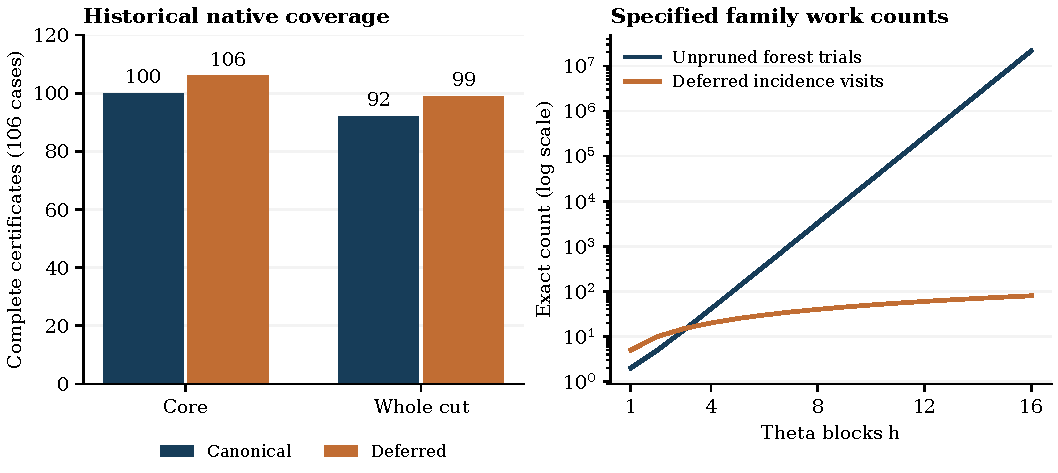
\includegraphics[width=\textwidth]{figures/research_results.pdf}
\caption{Left: exact historical certificate counts, separating cores
from whole cuts.  Right: the proved number of forests tested by the
specified unpruned family enumerator and the number of deferred incidence
visits.  The right panel compares exact work counts of different kinds;
it is not a universal lower bound or a wall-clock speedup chart.}
\label{fig:results}
\end{figure}
\FloatBarrier

% Article fragment. Requires amsmath, amssymb, amsthm and environments
% lemma, proposition, corollary. Suggested bibliography key: Hempel1976.
% The classical handlebody criterion below is not claimed as a new theorem.
\section{A terminal recognition route through free fundamental groups}
\label{sec:terminal-free-group}

The raw cancellation algorithms deliberately recognise a restricted
certificate class.  A different terminal certificate can use the
fundamental group, provided that irreducibility is already justified by
the source topology.  This permits algebraic certificates to establish an
\emph{abstract} handlebody conclusion without interpreting the algebraic
moves as geometric handle slides.  We work with compact PL manifolds and
locally flat, properly embedded surfaces; equivalent smooth conventions
give the same statements.

\begin{lemma}[Cutting along surfaces with boundary]
\label{lem:proper-cut-irreducible}
Let $M$ be a connected irreducible compact orientable three-manifold.  Let $S$ be a
finite disjoint union of compact, properly embedded, two-sided surfaces
such that every connected component of $S$ has nonempty boundary.  Then
every component of $M\mathbin{\backslash\!\backslash}S$ is irreducible.
No incompressibility hypothesis on $S$ is required.
\end{lemma}
\begin{proof}
An embedded sphere $\Sigma$ in the interior of a cut component gives an
embedded sphere in $\operatorname{int}M$ disjoint from $S$.  It bounds an
embedded ball $B$ in $M$.  Since $\partial B$ misses $S$, every connected
component of $S$ that meets $B$ must lie entirely inside $B$.  Such a
component cannot meet $\partial M$, contradicting its nonempty boundary
and proper embedding.  Thus $B\cap S=\varnothing$.  Choosing the regular
neighbourhood used for cutting sufficiently small, $B$ lies in the cut
component containing $\Sigma$.  Changing this neighbourhood only changes
the cut by a collar isotopy, so the conclusion holds for the given cut.
\end{proof}

The hypothesis about components is necessary for this argument.  Cutting
a ball along an interior sphere produces a component homeomorphic to
$S^2\times I$, which is not irreducible.  If closed cutting surfaces are
allowed, irreducibility of their complementary pieces needs a separate
justification.

The next implication is classical; see Hempel~\cite{Hempel1976}.  We
include its standard compression argument to make the precise hypotheses
and the terminal use explicit.

\begin{proposition}[Classical free-group handlebody criterion]
\label{prop:free-group-handlebody}
Let $N$ be a compact connected orientable irreducible three-manifold with
$\partial N\ne\varnothing$.  If $\pi_1(N)\cong F_g$, the free group of
rank $g\ge0$, then $N$ is a handlebody of genus $g$.  In particular,
$g=0$ implies that $N$ is a three-ball.
\end{proposition}
\begin{proof}
If a boundary component $F$ has positive genus, the homomorphism
$\pi_1(F)\to\pi_1(N)$ cannot be injective: subgroups of free groups are
free, whereas a closed orientable positive-genus surface group is not
free.  The Loop Theorem therefore supplies a properly embedded disk
$D\subset N$ with $\partial D$ essential in $F$.

Cutting along $D$ preserves irreducibility by
Lemma~\ref{lem:proper-cut-irreducible}.  Van Kampen's theorem gives
$\pi_1(N)=\pi_1(N_1)*\pi_1(N_2)$ when $D$ separates, and
$\pi_1(N)=\pi_1(N\mathbin{\backslash\!\backslash}D)*\mathbb Z$ when
it does not.  Consequently all cut components again have free
fundamental group.  Every component still has nonempty boundary.

This process terminates.  Indeed, for the current union $W$ of components
define
\[
 \mu(W)=\sum_{\substack{F\subset\partial W\\g(F)>0}}(2g(F)-1).
\]
Compression along an essential separating curve on a boundary component
decreases $\mu$ by one.  Compression along a nonseparating curve in that
component decreases it by two, except on a torus, where it decreases it
by one.  Thus every
disk cut strictly decreases this nonnegative integer.

At termination all boundary components are spheres.  A connected
irreducible three-manifold with a sphere boundary component is a ball:
push that sphere slightly into the interior and use the ball it bounds
on the side away from its boundary collar.  Hence all terminal components
are balls.  Reversing the disk cuts attaches one-handles to these balls,
and recovers a handlebody.  Its genus is $g$, since a genus-$g'$ handlebody
has fundamental group $F_{g'}$ and free-group rank is an isomorphism
invariant.
\end{proof}

\begin{corollary}[Source-bound terminal group certificates]
\label{cor:terminal-tietze}
Under the hypotheses of Lemma~\ref{lem:proper-cut-irreducible}, assume
additionally that $\partial M\ne\varnothing$, and let $N_i$ be the
connected components of the \emph{whole} cut.  Suppose a source
verifier reconstructs a presentation $\mathcal P_i$ of $\pi_1(N_i)$, and
an algebraic verifier certifies
\[
 \mathcal P_i\ \cong\ \langle y_1,\ldots,y_{g_i}\mid\ \rangle
\]
for every $i$.  Then the cut is a disjoint union of handlebodies of genera
$g_i$.  It is a disjoint union of balls exactly when every $g_i$ is zero.
\end{corollary}
\begin{proof}
Every $N_i$ is irreducible by the lemma, and has nonempty boundary because
the source and cutting surfaces have boundary.  The verified group
isomorphism and Proposition~\ref{prop:free-group-handlebody} give the
conclusion component by component.
\end{proof}

One possible algebraic certificate is a sequence of elementary Tietze
transformations from the authenticated presentation to the displayed
free presentation.  The checker must verify each transformation.  A
relator claimed to follow from earlier relators must carry an explicit
consequence witness, such as a product of conjugates; its validity cannot
be delegated to an unspecified group-word oracle.  Generator definitions,
relator inversions, conjugations, products, and their certified inverses
give familiar checkable building blocks.  If words are compressed, their
equality checks and all certificate sizes must be measured in that
encoding.  The initial presentation must describe the entire component,
including bundle gluing relations, rather than merely its source core.

This is a proposed terminal extension, not an additional implemented
success in the reported experiments.  Its use requires authenticated
irreducibility and the stated source identification.  It supplies neither
a meridian disk system in marked coordinates nor a boundary-pattern
transport map.  A positive free rank gives a handlebody rather than the
ball required at the end of an essential hierarchy; a boundary-pattern
essentiality test remains separate even when the underlying piece is a
ball.  Finally, the classical theorem and the existence of a finite
Tietze certificate provide no polynomial or quasi-polynomial bound on
finding such a certificate, or on its size.  These are separate research
questions.

% Bibliographic verification, retrieved 12 October 2026:
% John Hempel, 3-Manifolds, Annals of Mathematics Studies 86,
% Princeton University Press, 1976.
% The original book page was not directly inspected. The author-hosted
% Culler--Shalen preprint "Volumes of hyperbolic Haken manifolds, I"
% explicitly cites Hempel, Theorem 5.2, for the irreducible/free-pi1
% handlebody-or-S^3 criterion (printed p.16, PDF page index15), and its
% reference6 gives author/title/series/volume/publisher:
% https://homepages.math.uic.edu/~culler/papers/HyperHakenI/nonsep.pdf
% Accordingly the article cites Hempel without an uninspected theorem number.

\section{What would actually imply quasi-polynomial recognition?}
\label{sec:complexity}

The new results remove a local combinatorial obstruction to efficient
normalization.  They do not bound the number, size, or required geometry
of the states visited by a complete knot algorithm.  This section makes
the distinction quantitative, so that future work has a falsifiable
complexity target rather than an analogy with a fast local benchmark.

\subsection{A conditional composition theorem}

\begin{proposition}[Explicit accounting for a complete implementation]
\label{prop:composition}
Suppose a correct total unknot-recognition implementation on diagrams of
size $n$ makes at most $Q(n)$ calls to its geometric state-processing
operator.  Suppose all state encodings have size at most $N_*(n)$, every
exceptional interface has size at most $U(n)$, and all remaining work per
state, including certificate generation, geometric transport, and replay,
is bounded by a fixed polynomial in $N_*(n)+1$.  Allow at most
$(N_*(n)+1)^{O(1)}$ selector invocations per state, each on an input of
encoded size $(N_*(n)+1)^{O(1)}$.  Assume also that all work outside these
state calls, including preprocessing and finalization, is polynomial in
$n+N_*(n)+1$.  If it uses the exact finite selector of
Theorem~\ref{thm:exceptional-selector}, then its total time is bounded by
\begin{equation}
 T(n)\le (Q(n)+1)\,(n+N_*(n)+1)^{O(1)}
       2^{O(U(n)\log(U(n)+2))}.
 \label{eq:composition}
\end{equation}
In particular, the three bounds
\begin{align*}
 \log(Q(n)+2)&=O((\log(n+2))^2),\\
 \log(N_*(n)+2)&=O((\log(n+2))^2),\\
 U(n)\log(U(n)+2)&=O((\log(n+2))^2)
\end{align*}
suffice for $T(n)=n^{O(\log n)}$ for $n\ge2$.
\end{proposition}
\begin{proof}
Each finite selection costs at most a polynomial in its encoding times
the Bell-number factor.  The input-size hypothesis and the bound on the
number of invocations absorb all selector calls into the same fixed
polynomial factor per state.  Sum this and the remaining per-state costs
over at most $Q(n)$ calls, then absorb the outside work using $Q(n)+1$
and the polynomial in $n+N_*(n)+1$.  Taking logarithms gives terms bounded
by $\log(Q(n)+2)$, $O(\log(n+N_*(n)+1))$, and
$O(U(n)\log(U(n)+2))$.  Each is $O((\log n)^2)$ under the stated
hypotheses.  Exponentiating gives the conclusion.
\end{proof}

This is complexity accounting, not a new total-recognition theorem.
The first sentence assumes correctness and termination of a complete
implementation.  Our existing partial census procedure does not satisfy
that premise merely because every emitted certificate is correct.

A more convenient sufficient state-size condition is $N_*(n)=n^{O(1)}$.
Under this stronger condition, $U=O(\log n)$ gives local cost
\[
 2^{O(\log n\log\log n)}=n^{O(\log\log n)}.
\]
The weaker interface bound
$U=O((\log n)^2/\log\log n)$ also suffices for the target local
$n^{O(\log n)}$ estimate, away from small $n$.  Neither interface bound
is proved for arbitrary native inputs or along the required hierarchies.
The absence of a dependence exponential in the number of top handles
does not itself control $U$.

\subsection{Hierarchy depth, loop counts, and the displayed exponent}

The loop estimate $L(g+1)^L$ from Proposition~9.1 of
\cite{Lackenby2026} uses the maximum hierarchy length $L$ and the maximum
\emph{pattern complexity} $g$ of its decomposing surfaces.  This complexity
includes boundary-pattern intersections; a genus bound alone does not
control it.  The estimate immediately shows why quantitative depth
matters.  If $g\le n^a$ and $L\le b\log n$, then
\[
 \log\bigl(L(g+1)^L\bigr)
 =\log L+L\log(g+1)=O((\log n)^2).
\]
If instead $L=O((\log n)^2)$ with the same pattern-complexity bound, this calculation
gives $O((\log n)^3)$ in the exponential, namely
$n^{O((\log n)^2)}$.  A bound merely linear in a handle-complexity
parameter that can itself be polynomial in $n$ does not give either
logarithmic-depth conclusion.

The purpose of comparing the two 2021 slide estimates is therefore
specific: an implementation and proof should state which exponent they
establish.  Replacing a polynomial local factor by a faster polynomial
does not repair an uncontrolled hierarchy depth.  Conversely, a
quasi-polynomial number of states can still tolerate another
quasi-polynomial local factor of the same logarithmic exponent, as
Proposition~\ref{prop:composition} shows.

\subsection{Encoding is part of the theorem}

Let $t$ count the source tetrahedra, and let $b$ be the total bit length
of the supplied normal coordinates.  A local source-to-certificate bound
should be expressed in $t+b$ and in the encoded marked interfaces it
creates.  It should not hide a scan through $W$ parallel sheets behind a
phrase such as ``construct the cut.''  The distinction is familiar from
the orbit-counting machinery of Agol--Hass--Thurston
\cite{AgolHassThurston}; its algorithmic value is that large multiplicities
can be processed through finite interval data.

The deferred theorem never requires expanding those sheets: it operates
on a supplied finite incidence matrix.  But this does not prove that
every matrix needed later in a hierarchy will have small encoded size.
Annular paths, port refinements, boundary patterns, and repeated chart
substitutions can dominate the size even when scalar multiplicities
remain in binary.  Every successor operator therefore needs an explicit
bound on both the number of records and the bits in each record.

Output size creates an independent barrier.  If a cut has exponentially
many identical ball components, writing one certificate per component
cannot take polynomial time in a binary multiplicity.  The existing
census representation groups such components by genus and multiplicity.
A full hierarchy certificate needs an equally explicit policy for
sharing repeated local structures and for authenticating that sharing.

\subsection{Outstanding geometric and algorithmic obligations}

The known local hierarchy theorems cited in Section~\ref{sec:scope} are
valuable starting points.  The following are the stronger or
implementation-specific obligations still absent from this package.

\begin{enumerate}
\item \emph{Controlled progress.}  Produce the decomposing multisurfaces
or other accelerated progress objects needed for a short global
construction, and prove their depth and pattern-complexity bounds,
including boundary-pattern intersections, in the actual source encoding.
Finding an arbitrary nonseparating surface is not the open
subproblem here.
\item \emph{Source-authenticated successor transport.}  Implement the
applicable compressed cutting and parallelity constructions with explicit
marked boundary maps, preserving the hypotheses needed for the next
state.  A census is less information than a successor handle structure.
\item \emph{Repair and restart accounting.}  Bound all branches caused
by unsuccessful local candidates, changes of charts, boundary-pattern
repairs, or restarts.  Charging only successful cuts omits real work.
\item \emph{A complete terminal procedure.}  The raw certificate class
is not complete for all handlebodies in arbitrary charts.  A total
algorithm must explain what happens after a universal raw obstruction,
and bound the cost of its alternative.  It must also decide the relevant
boundary-pattern condition, not just whether the underlying pieces are
balls.
\item \emph{Exceptional-interface control.}  Bound $u$, replace it by a
more stable parameter, or find a polynomial selector for the actual
geometric class.  The abstract triangle witness prevents one particularly
simple invariance argument but does not settle that geometric question.
\end{enumerate}

These obligations interact.  A move that reduces $u$ while making marked
paths exponentially long may lose overall.  A normalization that reduces
the number of records but changes the admissible pattern may invalidate
the next theorem.  The intended measure must charge both geometry and
encoding, with a source verifier checking each claimed transition.

\subsection{Algebraic simplification and geometric transport}

Whitehead minimization has polynomial algorithms in the length of
explicitly written free-group words \cite{RoigVenturaWeil}.  Such a bound
is not automatically polynomial in the size of a compressed grammar for
those words.  More fundamentally, an algebraic automorphism does not by
itself give the marked meridian and port data expected by the native
geometric kernel.  The recent thickenable-presentation work
\cite{LackenbyStable2026} provides relevant structural context, but no
bounded marked-slide implementation is supplied here.

Section~\ref{sec:terminal-free-group} gives a legitimate alternative
use: under authenticated irreducibility hypotheses, a verified free
fundamental group proves an abstract terminal handlebody.  It can bypass
the need to interpret each algebraic transformation as a slide when only
that terminal conclusion is required.  It still needs a bound on the
source presentation, the certificate, and its discovery.  It also cannot
be substituted for marked transport when the algorithm must continue.

\section{A proposed research programme}
\label{sec:research}

The most useful next steps should either remove a named asymptotic
obstruction or produce an independently checkable new geometric success.
The questions below are ordered by their likely value to this codebase.
They are proposals, not conjectures silently used in the proofs above.

\subsection{Immediate implementation and diagnostic work}

\paragraph{1. Authenticate the exceptional selector on native inputs.}
Build the missing adapter for Corollary~\ref{cor:coupled-forests}.  Export
the full pre-primal occurrence matrix and source dual endpoints, mark
nonselectable rows, run the finite selector, and feed the resulting tree
through the existing geometric reduction.  Reuse the ordinary source
verifier for every positive packet.  The initial acceptance criterion is
correct transport and equality with exhaustive dual-tree enumeration on
small native cores, followed by a source-authenticated example where
dual choice adds coverage after deferred primal selection.  A synthetic
matrix success is insufficient for this milestone.

\paragraph{2. Resolve the remaining literal handlebody example.}
The fixture \path{pilot/finite_figureEight/0} is the only all-handlebody
whole cut missed among the 113 completed literal oracle comparisons.
Its components have genera one and two.  Determine the exact obstructing
annular or augmented relation and produce the smallest checkable repair.
First establish which geometric and irreducibility hypotheses apply;
then compare a supported slide certificate, a group-based terminal
certificate, or a change of dual reduction where one exists.  This is a
concrete native target for moving beyond raw stopping sets.

\paragraph{3. Implement an adaptive canonical/deferred policy.}
Can the canonical fast path be retained without paying twice for source
construction when it stalls?  Share immutable full rows and source
component data; run canonical peeling as a view or maintain enough
deleted-column metadata to retry deferred discovery.  Measure source
preparation, producer time, replay, allocation, and certificate size
separately.  The target is to preserve the historical common-success
latency while retaining all nine new whole-cut results.  Keep the simple
opt-in path available as a reference implementation.

\paragraph{4. Export and minimize universal primal obstructions.}
The greatest stopping residual is canonical for a fixed matrix, but it
need not be the smallest witness.  Find small source-bound stopping
subsets for diagnosis and caching.  Determine whether minimum-cardinality
or minimum-support stopping witnesses are tractable in the actual native
class.  A heuristic minimizer is useful if an independent checker verifies
its result.  Every cache key must retain source identity, retained rows,
and the raw occurrence convention.

\subsection{Sharper finite algorithms}

\paragraph{5. Replace Bell enumeration by representative families.}
The completeness proof needs at most $u$ additional tree witnesses.
Can a representative-family construction in the graphic matroid preserve
all useful interface signatures and reduce the $2^{O(u\log u)}$ factor
to $2^{O(u)}$, or give a small kernel?  Any such reduction must preserve
both nonlinear Horn closure and simultaneous independence with the
mandatory representatives.  Keeping one edge per signature is not
obviously safe: equal activation signatures can have different graphic
dependence with the chosen forest.

\paragraph{6. Parameterize the compressed rule interaction instead of $u$.}
Construct the bipartite graph of exceptional rules and interface rows,
or the incidence graph after baseline strongly connected components are
contracted.  Investigate dynamic programming by treewidth, branchwidth,
or separator size while retaining the graphic-independence constraint.
A useful theorem should specify its states and account for connectivity
partitions; otherwise a hidden Bell-number factor can reappear in each
bag.  The native cycle condition may constrain this graph more strongly
than arbitrary hypergraph activation.

\paragraph{7. Settle the genuinely native triple-column problem.}
The saved nine-vertex witness refutes tree invariance from sparsity and
dual-cycle parity alone.  Which additional constraints imposed by an
actual triangulated normal cut exclude it, if any?  Either construct a
native realization preserving the required ports, or prove a stronger
geometric restriction and exploit it algorithmically.  This would decide
whether the remaining selector should be studied as a general constrained
activation problem or as a substantially narrower topological class.

\paragraph{8. Make exhaustive dual failure independently checkable.}
For one partial partition, matroid intersection can expose a rank defect.
Can the failures of all partitions be compressed into a small certificate
that covers the entire search space, perhaps by shared Horn-closure
states and reused rank inequalities?  The objective is a certificate
for failure of the finite raw model, not a nonunknot certificate.  A
worst-case size bound would be more valuable than merely logging the
full exponential enumeration.

\paragraph{9. Analyze the best parameter after legal simplification.}
The theorem uses exceptional rows in the input before unknown dual
deletions.  Study the minimum achievable exceptional size under cheaply
certified preprocessing, preserving the exact forest-selection problem.
Possible reductions include automatic-seed closure, domination of Horn
rules, irrelevant-column removal, and decompositions with independently
tracked graphic constraints.  Prove equivalence for each reduction;
deleting a row because it would become useful in some unknown tree is
not valid preprocessing.

\subsection{Geometry beyond the current raw model}

\paragraph{10. Certify marked slides that decrease an explicit potential.}
Define a potential combining raw intersection size, exceptional support,
and encoded port length.  Seek a class of geometric one/two-handle
slides for which a verifier reconstructs the actual band and proves a
controlled decrease or bounded amortized increase.  The theta family
shows that forest choice alone can suffice in some cases; the remaining
whole-cut example asks for a move beyond that theorem.  Algebraic
relator shortening is a guide, not the marked geometric certificate.

\paragraph{11. Develop the terminal free-group certificate route.}
For cuts satisfying the boundary and irreducibility conditions of
Section~\ref{sec:terminal-free-group}, construct authenticated whole-cut
presentations and short Tietze or Nielsen certificates of freeness.
Determine which existing compressed words admit polynomial equality
checking and whether the certificate construction stays within that
encoding.  Separate three questions: proving the group is free,
recovering an abstract genus, and recovering a marked disk system.
Only the first two are needed for the terminal implication proved here.

\paragraph{12. Realize the deferred-basis theorem geometrically.}
The represented-matroid extension preserves column span but does not
make every basis a collapsible subcomplex.  Identify a class of regular
cell structures in which the discovered basis has a certifiable
geometric realization, or characterize the additional obstruction.
This may connect the graph proof to higher boundary operators without
confusing homological independence with simple-homotopy or handle
cancellation data.

\subsection{The global quasi-polynomial programme}

\paragraph{13. Prove an interface budget along accelerated hierarchies.}
Can each maintained state be transformed, with bounded marked cost, to
one satisfying $u\log(u+2)=O((\log n)^2)$?  A weaker amortized theorem
bounding the sum of per-state costs could also suffice.  Measure $u$
together with handles, ports, coordinate bits, genus, and source-grammar
size on successive authentic cuts before conjecturing a logarithmic
law.  A logarithmic observation in a small corpus is not an asymptotic
bound.

\paragraph{14. Build the complete marked successor operator.}
Implement the applicable compressed successor constructions as a total
source-to-source certificate step under their geometric hypotheses.
Record handles, boundary patterns, attaching maps, inherited markings,
parallelity data, and all reindexing maps.  Prove a uniform encoding
bound under composition.  This is the central bridge from successful
terminal censuses to an actual hierarchy engine.

\paragraph{15. Bound depth, repairs, and terminal completion together.}
Formulate one theorem with all quantities in
Proposition~\ref{prop:composition}: the state-call count $Q(n)$, encoding
size $N_*(n)$, exceptional parameter $U(n)$, and a complete terminal
procedure.  Surface construction should target the stronger controlled
progress needed for the announced speed-up.  Include unsuccessful
candidate work and boundary-pattern repairs in the accounting.  The
decisive milestone is a proved bound for a correct total algorithm,
not a collection of separately fast routines.

\paragraph{16. Formalize the finite invariants before the full topology.}
The stopping-set invariant, deferred graph forest theorem, represented
binary-matroid extension, and compressed Horn reduction are finite,
explicit statements with short constructive proofs.  They are good
initial targets for proof-assistant formalization or small verified
checkers.  Formalizing these layers would reduce the trusted combinatorial
base while geometric source-authentication proofs continue separately.
The supplied counterexamples and mutation cases are regression fixtures
for that formalization, not substitutes for it.

The recommended order is to complete the native adapter and adaptive
implementation while pursuing the exceptional-interface and marked
successor questions in parallel.  The article's strongest established
asymptotic gain is already unconditional within its finite geometric
model: primal forest enumeration is unnecessary.  The next global
advance must control the state evolution that feeds those local models.

\appendix
\section{Package contents and reproduction}
\label{app:reproduction}

The package is an integration bundle for the source snapshot
\cite{RepoSnapshot}.  It contains the article's complete \TeX{} source,
compiled PDF, bibliography, and figure source; an additive patch and
six-file overlay; the independent finite research operator; source-bound
positive packets; raw audit/timing data; and reproduction commands.
The repository itself and third-party papers are not duplicated.

\begin{table}[htbp]
\centering\small
\begin{tabular}{p{0.28\textwidth}p{0.63\textwidth}}
\toprule
Directory or file & Purpose\\
\midrule
\code{article/} & Master \TeX, section files, bibliography, PDF, and figure.\\
\code{patches/} & Patch against the pinned baseline.\\
\code{overlay/} & The same six changed source/test files, with repository-relative paths.\\
\code{baseline/} & Original versions of the four changed production modules.\\
\code{finite\_selector/} & New exceptional solver, attributed prior backend, independent exhaustive checker, and triangle witness.\\
\code{certificates/} & Nine whole-cut and eight core packets, retaining their source inputs.\\
\code{tools/} & Audit, replay, benchmark, and plotting drivers.\\
\code{results/} & Raw measurements, complete audit counts, regression recovery, and source validation records.\\
\code{SOURCE\_AUDIT.json} & Baseline, hashes, environment, and change provenance.\\
\code{CLAIMS.json} & Machine-readable result and limitation ledger.\\
\code{SHA256SUMS} & Integrity hashes for the delivered files.\\
\bottomrule
\end{tabular}
\caption{Integration bundle layout.}
\end{table}

\subsection{Build the article}

From the package root:
\begin{Code}
cd article
latexmk -pdf -interaction=nonstopmode -halt-on-error \
  Deferred_Forests_and_Exceptional_Incidence.tex
\end{Code}
The supplied \code{build.sh} performs this command.  The figure PDF is
already included.  Regenerating it with \code{tools/generate\_figures.py}
requires Matplotlib; compiling the article does not require Python.

\subsection{Apply and exercise the native change}

Check out the pinned revision or inspect the patch carefully against a
later tree.  From the repository root, using an absolute package path:
\begin{Code}
git apply --check /path/to/package/patches/deferred_forests.patch
git apply /path/to/package/patches/deferred_forests.patch
cd Topology/UnknotRecognition/fast
python3 -m unittest tests.test_deferred_forest \
  tests.test_deferred_boundary_kernel -v
\end{Code}
These tests require the source fixtures and Regina used by the native
project.  Full discovery also needs the historical reference modules
documented in the recovery log; a checkout containing only \code{fast}
is not sufficient for that broader suite.

An actual call uses the same source data as before:
\begin{Code}
result = normal_cut_handlebodies(
    triangulation, coordinates,
    record_certificate=True,
    forest_strategy='deferred',
)
if result['status'] == 'COMPLETE':
    assert verify_normal_cut_handlebodies(
        triangulation, coordinates, result['certificate'])
\end{Code}
The import statements and a runnable packet-replay command appear in the
package README.  Callers must retain the \code{INCONCLUSIVE} distinction.

\subsection{Reproduce the finite theorem audit}

No topology library is required for the standalone operator:
\begin{Code}
cd finite_selector
python3 audit_exceptional.py --output audit_results_new.json
python3 check_triangle_witness.py
python3 exceptional_forest.py examples/triangle.json
\end{Code}
The complete audit seeds, instance classes, literal oracle, and budget
checks are recorded in its source and README.  Native whole-cut replay
and timings have explicit \code{--fast-root} arguments so they can be
run against an isolated patched checkout.  The article's values are
fixed measurements; a new run should write a new result file instead of
silently replacing the delivered evidence.

\subsection{Reproducibility limits}

The test suite is extensive but not a formal proof of implementation
correctness.  The mathematical proof is independent of the observed
sample counts.  The standalone audits range over finite graph/matrix
instances and do not establish native geometric realizability.  The
literal oracle comparisons exclude inputs beyond their expansion cap.
The source-bound packets and raw data allow each of these claims to be
rechecked separately, with their original scope intact.

\section{Complete data for the triangle sensitivity witness}
\label{app:triangle-data}

This appendix specifies the finite object in
Proposition~\ref{prop:exceptional-triangle-witness} without requiring an
external data file.  The graph vertices are $0,\ldots,8$.  Rows are the
25 edge labels below.  Each of the 17 Boolean matrix columns has value
one on its listed three rows and zero elsewhere.

\begin{table}[htbp]
\centering\small
\begin{tabular}{rl@{\qquad}rl@{\qquad}rl}
\toprule
Row & Endpoints & Row & Endpoints & Row & Endpoints\\
\midrule
0 & $(0,1)$ & 9 & $(1,8)$ & 18 & $(4,7)$\\
1 & $(0,2)$ & 10 & $(2,4)$ & 19 & $(4,8)$\\
2 & $(0,3)$ & 11 & $(2,5)$ & 20 & $(5,6)$\\
3 & $(0,4)$ & 12 & $(2,6)$ & 21 & $(5,7)$\\
4 & $(0,6)$ & 13 & $(2,7)$ & 22 & $(5,8)$\\
5 & $(0,7)$ & 14 & $(3,4)$ & 23 & $(6,8)$\\
6 & $(1,2)$ & 15 & $(3,7)$ & 24 & $(7,8)$\\
7 & $(1,6)$ & 16 & $(3,8)$ &  & \\
8 & $(1,7)$ & 17 & $(4,6)$ &  & \\
\bottomrule
\end{tabular}
\caption{Dual graph edge records.}
\end{table}

\begin{table}[htbp]
\centering\small
\begin{tabular}{rl@{\qquad}rl}
\toprule
Column & Supported rows & Column & Supported rows\\
\midrule
0 & $\{0,1,6\}$ & 9 & $\{11,12,20\}$\\
1 & $\{0,4,7\}$ & 10 & $\{11,13,21\}$\\
2 & $\{1,3,10\}$ & 11 & $\{14,15,18\}$\\
3 & $\{2,5,15\}$ & 12 & $\{15,16,24\}$\\
4 & $\{3,4,17\}$ & 13 & $\{17,19,23\}$\\
5 & $\{3,5,18\}$ & 14 & $\{18,19,24\}$\\
6 & $\{6,8,13\}$ & 15 & $\{20,22,23\}$\\
7 & $\{7,9,23\}$ & 16 & $\{21,22,24\}$\\
8 & $\{8,9,24\}$ &  & \\
\bottomrule
\end{tabular}
\caption{All 17 triangle columns, in the order used by the stopping totals.}
\end{table}

The successful and failing trees, respectively, are
\begin{align*}
T_+&=\{5,7,10,14,17,19,21,22\},\\
T_-&=\{1,2,5,8,12,16,19,20\}.
\end{align*}
A successful trace on the complement of $T_+$ consists of the following
$(\text{row},\text{column})$ pairs in order:
\[
\begin{gathered}
(23,13),\ (9,7),\ (20,15),\ (24,16),\ (8,8),\ (18,14),\\
(3,5),\ (1,2),\ (4,4),\ (0,1),\ (6,0),\ (13,6),\\
(11,10),\ (12,9),\ (15,11),\ (2,3),\ (16,12).
\end{gathered}
\]
For $T_-$ the recorded legal prefix is
\[
\begin{gathered}
(15,3),\ (11,9),\ (24,12),\ (9,8),\\
(18,14),\ (3,5),\ (10,2),\ (14,11).
\end{gathered}
\]
The remaining rows are $\{0,4,6,7,13,17,21,22,23\}$.  Directly summing
the displayed columns on this set gives
\[
(2,3,0,0,2,0,2,2,0,0,2,0,0,2,0,2,2),
\]
a nonempty stopping set with no unit total.  Checking each three-edge
column against the endpoint table verifies that it is a graph triangle.
The independent checker in the package repeats precisely these finite
checks, without invoking the exceptional solver or a topology library.


\bibliographystyle{plain}
\bibliography{references}
\end{document}
